\chapter{Object Definition and Reconstruction}
\label{sec:obj}

The previous chapter described how the ATLAS detector collects information on 
final state particles produced in $pp$ collisions in the form of,
for example, hits in the Inner Detector and Muon Spectrometer
or energy deposits in the calorimeter.
This chapter defines physics objects,
which are observables that allow us to study the hard-scatter processes and
form the basis of the analyses in future chapters.
This chapter will describe how, using the information provided by the ATLAS detector,
each physics object is identified
and their 4-momentums and trajectories reconstructed.

Specifically this chapter will focus on physics objects important to the analyses in this thesis:
tracks are described in Section~\ref{sec:obj-tracks}, jets in Section~\ref{sec:obj-jets},
$b$-jets in Section~\ref{sec:obj-bjets}, and electrons and muons in Section~\ref{sec:obj-leptons}.
Finally, Section~\ref{sec:obj-further} will briefly describe some further physics objects
widely used in the ATLAS physics program outside of the analyses being presented here.

\section{Tracks}
\label{sec:obj-tracks}

The ATLAS detector is able to reconstruct the trajectory of charged particles produced
in the proton-proton collision as they pass through the Inner Detector;
the reconstructed trajectories are known as tracks.
Track reconstruction is essential in a number of important areas of ATLAS analyses:
for example; primary vertex reconstruction, identification of $b$-jets (Section~\ref{sec:obj-bjets})
and the identification and reconstruction of electrons and muons (Section~\ref{sec:obj-leptons}).

Track reconstruction uses hits from the Pixel detector, SCT and TRT which are described in Section~\ref{sec:det-ID}.
The track reconstruction is performed using an `inside-out' approach,
which entails using the higher precision Pixel and SCT hits initially
before adding in the TRT hits to improve track quality.
The tracking reconstruction procedure~\cite{obj-tracks_TIDE} follows these steps:
\vspace{-0.5em}
\begin{itemize}[leftmargin=*]
\item\textbf{Clustering:}
  \footnote{In the associated reference this step is referred to as `clusterization', but here I will use clustering for consistency with the English language.}
  Neighbouring hits in a layer of the Pixel or SCT detector are converted into a 3D `space-point'
  that represents the point where the charged particle traversed the active material of the ID.
  In the Pixel detector one cluster of hits can form a space-point,
  whilst in the SCT hits from both sides of a strip layer are required to create a 3D space-point.\vspace{0.5em}
\item\textbf{Track Seeding:}
  Track seeds are formed from three space-points in consecutive layers of the Inner Detector
  that are consistent with the trajectory of a particle with $p_T >$ 500 MeV.\vspace{0.5em}
\item\textbf{Track Candidates:}
  From the track seeds, track candidates are built by iteratively adding space-points
  from the remaining Pixel and SCT detector layers using an combinatorial Kalman filter~\cite{obj-tracks_kal}.
  There can be multiple track candidates per seed.\vspace{0.5em}
\item\textbf{Track selection / Ambiguity resolving:}
  Each track candidate is assigned a `track-score' that is based a number of variables of the track candidate;
  the $p_T$, $\eta$, $\chi^{2}$ fit and the hit pattern.
  The hit pattern refers to the number of Pixel or SCT hits,
  the number of holes (missing hits where one was expected)
  and the quality of the hits.
  Track candidates must also pass some track quality requirements,
  that are similarly based on the track candidate's $p_T$, $\eta$ and the hit pattern.
  The self-consistent set of track candidates that have the highest `track-score' and that pass track quality requirements are then selected.
  Exact details of the track-scoring, track requirements and selection algorithm is described in~\cite{obj-tracks_TIDE}.\vspace{0.5em}
\item\textbf{Add TRT Information:}
  Track candidates from the previous step are extrapolated into the TRT and all hits within \SI{10}{\milli\metre} are added.
  The track candidates are then refitted using Pixel, SCT and TRT hits to make use of the full tracking detector.
\end{itemize}

The outputs of the above track reconstruction process will be referred to as tracks in the remainder of this thesis.
Also it is important to note that, as discussed in Section~\ref{sec:det-ID}, the tracks are curved by a known magnetic field in the Inner Detector,
therefore the tracks contain information on the charge and the momentum of the particles whose trajectory they are describing.

\section{Jets}
\label{sec:obj-jets}

If a collision results in a free quark or gluon in its final state then a stream of high-energy hadrons is created,
which is known as a hadronic jet.
The underlying processes in hadronic jet formation can be summarised as follows;
firstly the free quark/gluon will radiate additional gluons and quarks in a process known as the parton shower,
these gluons and quarks will then undergo hadronisation to form hadrons which are the constituents of the hadronic jet.
A more detailed description of the parton shower and hadronisation process can be found in Section~\textit{[QCD theory description] Not written yet} \textbf{LM fix}.
The components of the hadronic jet deposit energy in the cells of the ATLAS calorimeter, through the processes described in Section~\ref{sec:det-calo},
such that the ATLAS calorimeter has an energy and positional measurement of the components of the hadronic jet.
The process of parton shower, hadronisation and energy deposition in the calorimeter, as described above, is illustrated in Figure~\ref{fig:obj-jets_schem}.

\begin{figure}[!ht]
  \begin{center}
    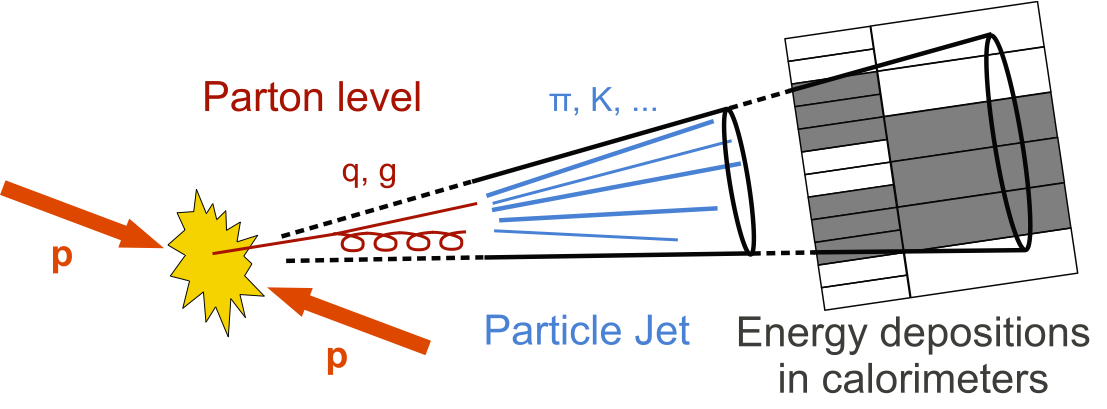
\includegraphics[width=0.8\linewidth, angle=0]{figs/Objects/jets_schem.png}
  \end{center}
  \caption[A schematic illustrating the formation of hadronic jets and the resulting observed energy deposits in the calorimeter system.]
          {A schematic illustrating the formation of hadronic jets and the resulting observed energy deposits in the calorimeter system \cite{obj-jets_schem}.}
  \label{fig:obj-jets_schem}
\end{figure}

This section contains a description of the procedure utilised by ATLAS
to go from energy deposits in calorimeter cells to well defined and calibrated hadronic jets.
This procedure can be split up into three separate steps that are described in the following sections;
firstly topoclusters are formed as described in Section~\ref{sec:obj-jets_topo},
then jets are formed from topoclusters using reclustering algorithms as described in Section~\ref{sec:obj-jets_reco}
and finally Section~\ref{sec:obj-jets_calib} and Section~\ref{sec:obj-jets_uncert}
describes how the jets are calibrated and the relevant jet energy uncertainties are derived.

In this section the formation of hadronic jets constructed from calorimeter cells is described,
as this is the only jet object used in the context of the analyses presented in this thesis.
However, it is worth noting, that there are other types of jets used at ATLAS;
%jets are used to observe electrons and taus whilst
for example hadronic jets can also be constructed from tracks formed in the Inner Detector,
a technique that has been useful in dense environments~\cite{obj-Hbb}.

\subsection{Hadronic Topocluster Reconstruction}
\label{sec:obj-jets_topo}

The first step of jet building at ATLAS is the formation of 3D clusters, known as topoclusters, from groups of energy deposits in neighbouring calorimeter cells~\cite{obj-jets_topo}.
The calorimeter cells can be from either the EM or hadronic calorimeter systems,
which have a granularity given in Table~\ref{tab:det-calo_granularity}.
The algorithm employed makes use of the variable ``cell signal significance'' defined as, 
\begin{equation}
  \Large{S_{\text{cell}} = \frac{E_{\text{cell}}}{\sigma_{\text{noise,cell}}}}
\end{equation}
where $E_{\text{cell}}$ is the energy deposited in a cell
and $\sigma_{\text{noise,cell}}$ is the uncertainty due to noise in that cell.
The sources of noise in a calorimeter cell are described in Section \textbf{LM fix, need to have a noise section somewhere...}.
A large value of $S_{\text{cell}}$ ( $>$ 1 ) indicates that the energy deposit is likely due to a particle
depositing energy in the calorimeter rather than noise within the calorimeter.

\noindent
Using the value of $S_{\text{cell}}$, each calorimeter cell is labelled as follows
\begin{itemize}
\item If $|S_{\text{cell}}| > 4$: the cell is labelled a \textbf{seed} cell.
\item If $|S_{\text{cell}}| > 2$: the cell is labelled a \textbf{growth} cell.
\item If $|S_{\text{cell}}| > 0$: the cell is labelled a \textbf{boundary} cell.
\end{itemize}
Then the algorithms builds topoclusters as in the following steps,
\begin{enumerate}
\item A seed cell forms the centre of a new topocluster.
\item Neighbouring seed cells are added together to form one topocluster seed.
\item Then, growth cells neighbouring the topocluster are added.
\item Finally, boundary cells neighbouring the topocluster are added.
\end{enumerate}
Figure~\ref{fig:obj-topo_schem} illustrates an example of where the algorithm would form a topocluster and an example where it wouldn't.

The topoclusters are treated as massless objects,
such that the four-momentum of each deposit can be calculated using the sum of energy deposited in the topoclusters
and the $\eta-\phi$ position of the topocluster.
The constructed topoclusters and their four-momentums are then used as the inputs to the next step of jet reconstruction.

\begin{figure}[!hbt]
  \begin{center}
    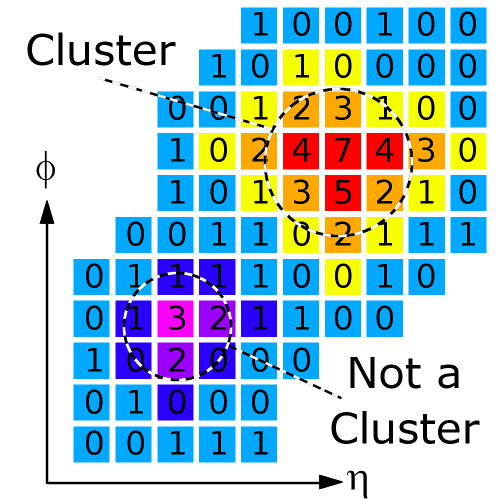
\includegraphics[width=0.7\linewidth, angle=0]{figs/Objects/topo_schem.png}
  \end{center}
  \caption[A schematic illustrating the algorithm used to form a topocluster. The numbers on the grid represent $|S_{\text{cell}}|$ and the colours represent the cell label.]
          {A schematic illustrating the algorithm used to form a topocluster. The numbers on the grid represent $|S_{\text{cell}}|$ and the colours represent the cell label~\cite{det-magnet_fig}.}
  \label{fig:obj-topo_schem}
\end{figure}

\FloatBarrier
\subsection{Jet Reconstruction}
\label{sec:obj-jets_reco}

The next step in the process is to form jets from the topoclusters described in the previous section.
To do this a jet reconstruction algorithm is defined,
that uses the location and energy of the topoclusters in an event to form a set of jets.
Each jet formed by the algorithm has a well defined four-momentum and set of constituents.
Jet reconstruction algorithms are used to define jets as this means that jets are experimentally well-defined model-independent observables,
which is required if measurements using jets are to be re-usable by the wider particle physics community.
A detailed discussion of jet reconstruction algorithms
and their related issues is found in~\cite{obj-jets_reco_salam};
as such this section provides a summary relevant to the analyses being presented in this thesis.

ATLAS analyses use a type of jet reconstruction algorithms known as sequential recombination algorithms,
which selectively add together the calorimeter topoclusters to form the jet;
these are specifically the $k_t$, anti-$k_t$ and Cambridge-Aachen (CA) algorithms.

The three algorithms use a set of four-momentums (clusters), which are initially the topoclusters formed in the calorimeter.
One then introduces an inter-jet distance between clusters $i$ and $j$ defined as,
\begin{equation}
  d_{ij} = \text{min}
  [(p_{ Ti})^a, (p_{ Tj})^a]  \left(\frac{\Delta  R_{ij}}{R}\right) ^2, \hspace{1cm} \Delta R_{ij} = \sqrt{(y_{i} - y_{j})^2 + (\phi_{i} - \phi_{j})^2} \label{dij}
\end{equation}
\noindent and a particle-beam distance for cluster $i$ defined as,
\begin{equation}
  d_{iB} = (p_{Ti})^a \label{diB}
\end{equation}
where $y$  is rapidity (as defined in Section~\ref{sec:det-coordinate}), $\phi$ is azimuthal angle,
$p_T$ is transverse momentum (component of momentum perpendicular to the beam-pipe of colliding particles)
and $p_z$ is the component of momentum that is parallel to the beam-pipe of colliding particles.
$R$ is the jet width parameter, a free parameter of the algorithm.
The parameter $a$ in Eq. \eqref{dij} and \eqref{diB} takes the value $a = 2$ for the $k_t$ algorithm, $a = -2$ for the anti-$k_t$ algorithm 
and  $a = 0$ for the Cambridge-Aachen algorithm.

The inter-jet and particle-beam distances are not physical distances as such, but can instead be thought of as dimensionful measures of how likely it is that
clusters $i$ and $j$ represent clusters caused by hadrons from the same jet.
If the inter-jet distance for a pair of clusters is smaller than the particle-beam distances for the two clusters ($d_{ij} < d_{iB}$) 
then it is likely that the two clusters are from the same jet. 
In contrast, if $d_{ij} > d_{iB}$ then it is unlikely that the two clusters are from the same jet.
 
\noindent The algorithm then proceeds using the following steps:
\vspace{-1em}
\begin{enumerate}[nolistsep]
  \item Calculate $d_{ij}$ and $d_{iB}$ for all combinations of clusters.  
  \item Find the minimum of the $d_{ij}$ and $d_{iB}$. 
  \item If the minimum is a $d_{ij}$ combine cluster $i$ and $j$ to form a new cluster and return to step 1. 
  \item If the minimum is a $d_{iB}$ then call cluster $i$ a final-state jet, remove it from the set and return to step 1.  
  \item Stop when all clusters have been declared as jets. 
\end{enumerate} 
The final jet has a four-momentum equal to the addition of all the topoclusters assigned to that jet.
It can now be seen that the jet width parameter, $R$, effectively gives the scale of the width of a reconstructed jet.
This is because when $\Delta R_{ij} > R$ for a pair of clusters,
$d_{iB} < d_{ij}$ for the cluster with the smaller value of ${p_T}$,
and thus the algorithm will not merge the two clusters.

The sequential reclustering algorithms described above are used as they satisfy two important theoretically motivated criteria:
infrared and collinear safety.
Infrared safety requires that the jet reconstruction algorithm result should be invariant against soft gluon emission \footnote{Soft means a low momentum}
and collinear safety requires that the jet reconstruction algorithm result should be invariant against a parton splitting into two partons with small angular separation.
These conditions are desirable as if the jet reconstruction algorithm is infrared or collinear unsafe,
two different sets of jets could be formed from identical hard-scatter processes
due to an additional emission process in the parton shower.
The sequential reclustering algorithms described above are infrared and collinear safe.
\footnote{Cone-based algorithms jet reconstruction algorithms used at some previous collider experiments,
  such as UA2 ~\cite{obj-jets_reco_UA2}, do not satisfy this infrared and collinear safety.}.

Anti-$k_T$ is the jet reconstruction algorithm used for the analyses being presented in this thesis, which is typical of analyses at ATLAS.
This is because the anti-$k_T$ algorithm provides regular jet shapes around the centre of the jet,
due to the fact that the algorithm reconstructs the high-$p_T$ core of the jets first and then adds in the lower $p_T$ suburbs in later steps.
Figure~\ref{fig:obj-jets_reco_shapes} shows the jets formed by the Cambridge-Aachen, $k_T$ and anti-$k_T$ algorithm using the same set of input clusters;
this illustrates that anti-$k_T$ algorithm creates more regular jet shapes than the other sequential-reclustering algorithms.
Further to this, the value of the jet width parameter is chosen as $R$=0.4,
which is consistent with the values suggested for gluon/quark jets in Section 5 of~\cite{obj-jets_reco_salam}
and is the standard value used in ATLAS analyses.

\begin{figure}[!ht]
  \captionsetup[subfigure]{aboveskip=-5pt,justification=centering}
  \begin{center}
    \subcaptionbox{Cambridge-Aachen} {
      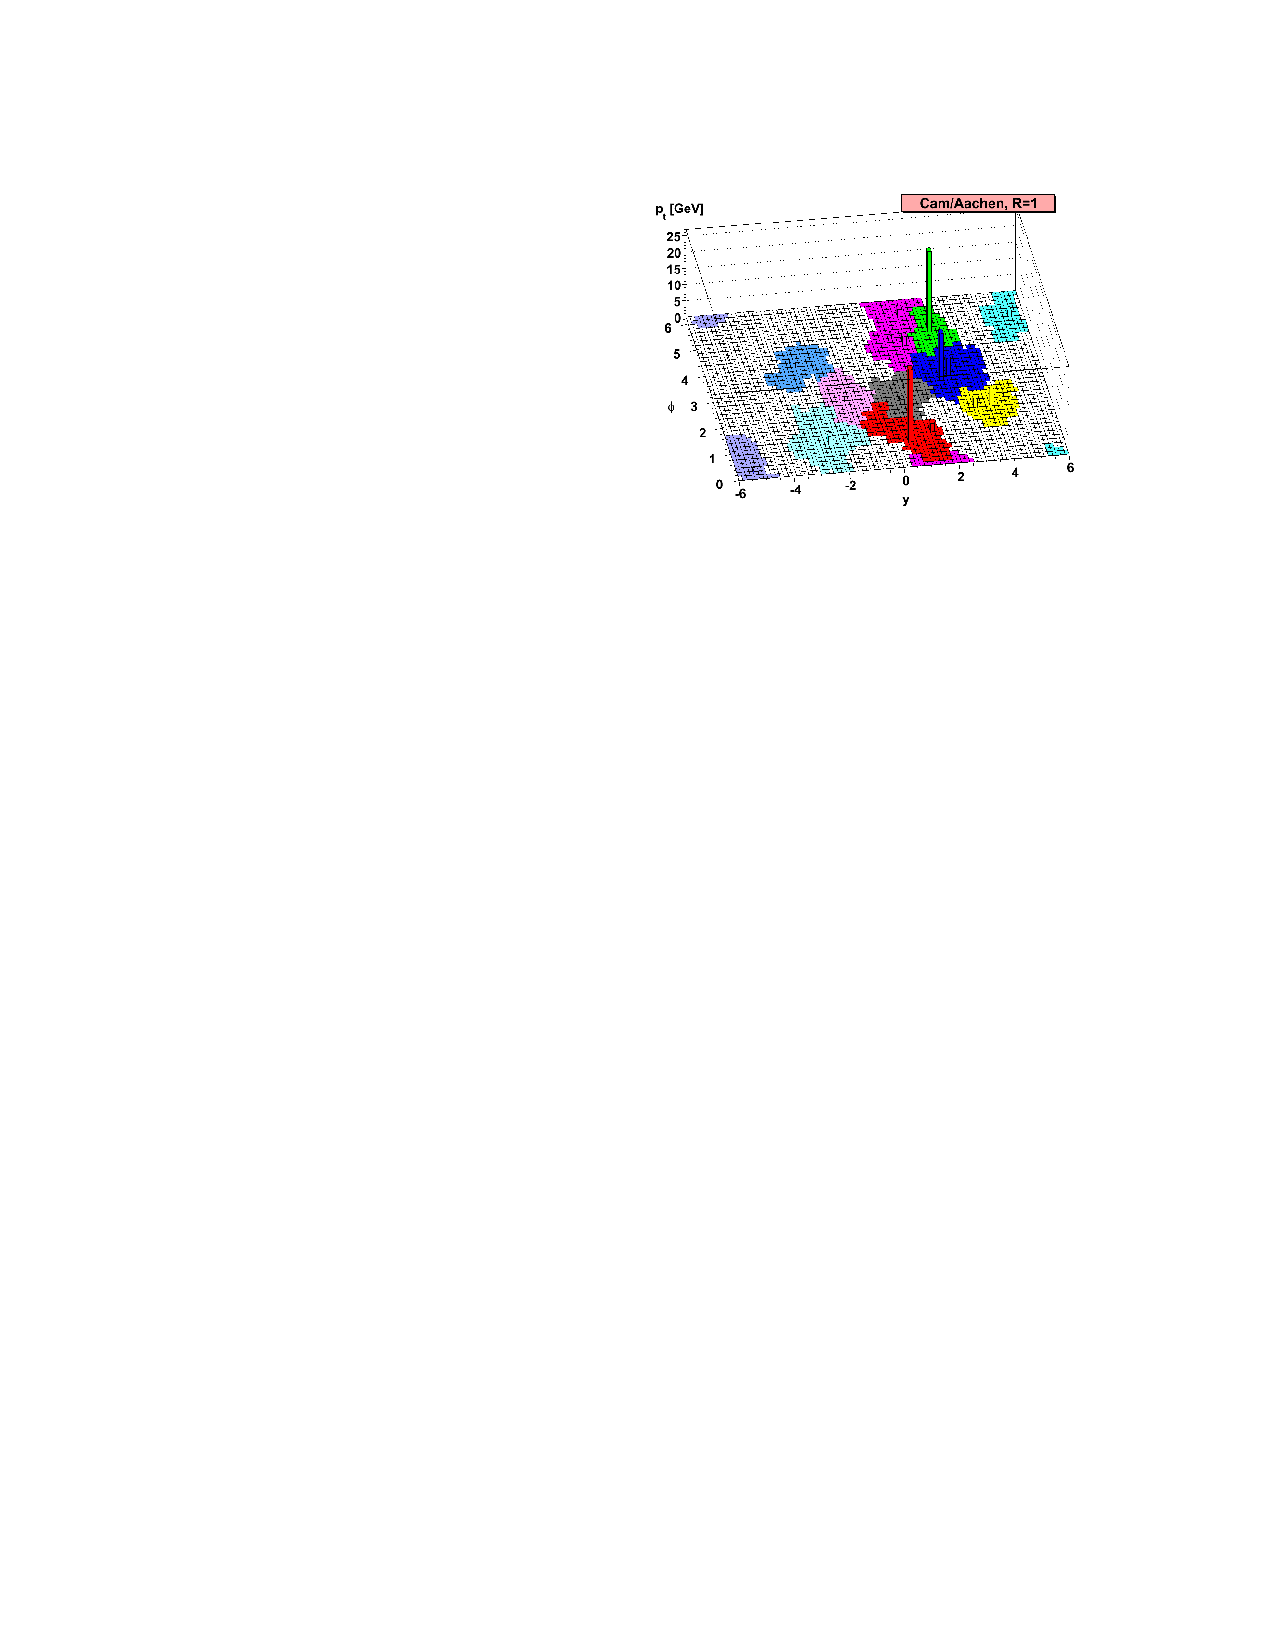
\includegraphics[width=0.45\linewidth, angle=0]{figs/Objects/jets_reco_shapes_ca.pdf}
    }
    \subcaptionbox{$k_T$} {
      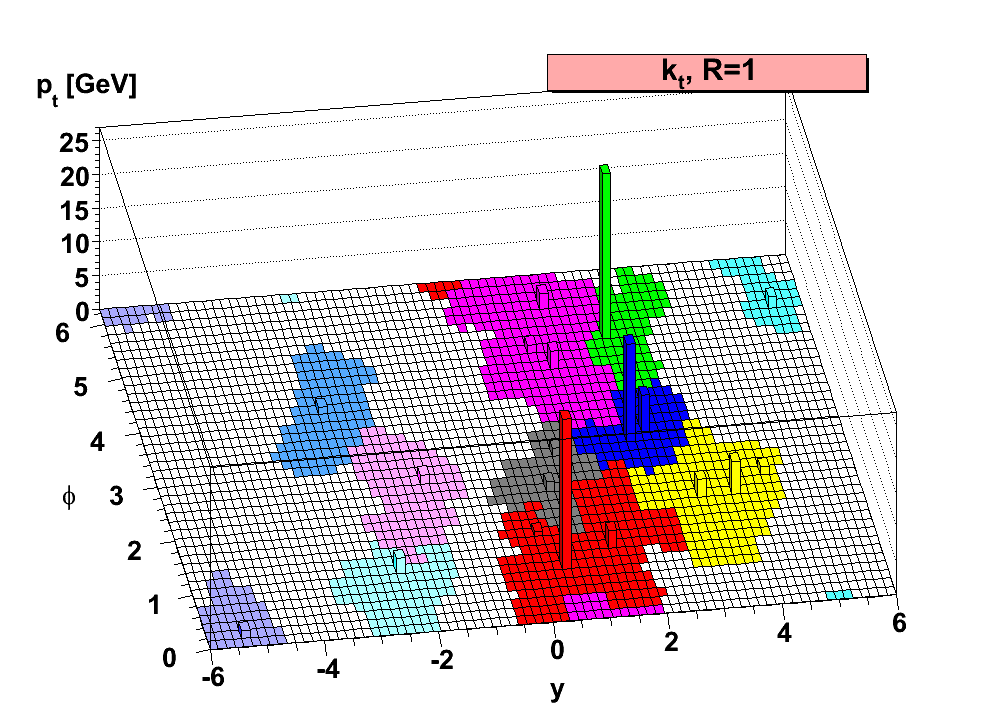
\includegraphics[width=0.45\linewidth, angle=0]{figs/Objects/jets_reco_shapes_kt.png}
    }\\
    \subcaptionbox{Anti-$k_T$} {
      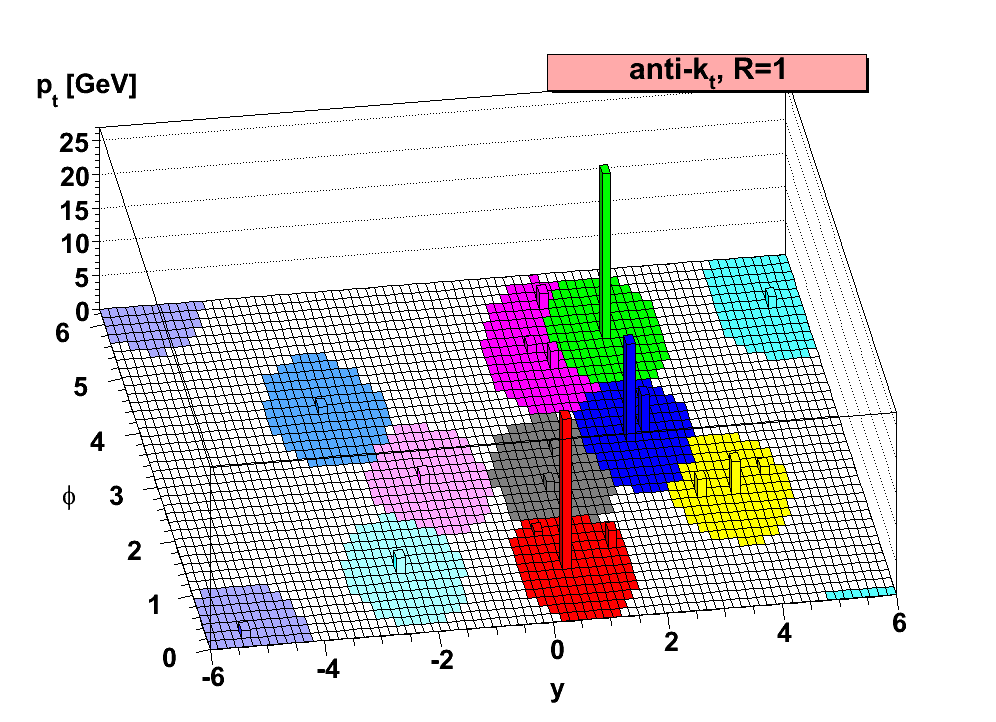
\includegraphics[width=0.45\linewidth, angle=0]{figs/Objects/jets_reco_shapes_akt.png}
    }

  \end{center}
  \caption[A comparison of the jets formed using the (a) Cambridge-Aachen, (b) $k_T$ and (c) anti-$k_T$ algorithm from the same simulated event.
    The constituent clusters of each of the jets formed is indicated using various colours.]
          {A comparison of the jets formed using the (a) Cambridge-Aachen, (b) $k_T$ and (c) anti-$k_T$ algorithm from the same simulated event.
            The constituent clusters of each of the jets formed is indicated using various colours \cite{obj-jets_reco_akt}.}
  \label{fig:obj-jets_reco_shapes}
\end{figure}

\subsection{Jet Calibration}
\label{sec:obj-jets_calib}

The jets initially formed by the jet reclustering algorithms from the topoclusters
will not represent the energy of the parton that initiated the parton shower (known as the initial parton)
and as such will not give an accurate dijet mass reconstruction which is required for the analyses presented in this thesis.
As a result, a hadronic jet calibration is required to map the initial reconstructed jet
to a more representative calibrated jet that can be used in an analysis.

\noindent
The key factors for the unrepresentative hadronic jet energy measurement are~\cite{det-thesis_kate,obj-jets_calib_2015}:
\begin{itemize}[leftmargin=*]
\item\textbf{Jet energy scale}:
  As discussed in Section~\ref{sec:det-calo_HCAL}, the ATLAS calorimeter is non-compensating which means that
  the calorimeter response is different for an EM-object and a hadronic object.
  The calorimeter response is calibrated at the EM-scale such that the energy measurements from a calorimeter cell
  are correct for an EM-object;
  as a result the initial energy measurement for a hadronic jet will be incorrect.
  To account for this a correction is required to take the jet energy measurement from the EM-scale to the hadronic-scale.\vspace{0.5em}
\item\textbf{Dead Material}:
  The hadronic jet may overlap with an unresponsive region of the detector,
  resulting in some energy deposits being incorrectly measured.\vspace{0.5em}
\item\textbf{Leakage}:
  Some energy from the jet will be distributed outside the angular acceptance of the calorimeter
  whilst some energy will pass through the calorimeter in a process known as `punch-through', as discussed in Section~\ref{sec:det-MS}.\vspace{0.5em}
\item\textbf{Reconstruction Issues}:
  There are two issues with jet reconstruction that require correction:
  firstly, some energy deposits coming from the initial parton may not be constructed as topoclusters due to the cell signal significance thresholds required in topocluster formation.
  Secondly, some topoclusters that should be clustered to the jet may not included in the reconstructed jet or included in a different jet instead.\vspace{0.5em}
\item\textbf{Pile-up}:
  Energy from collisions other than the hard-scatter collision can also be included by the reclustering algorithm.
  This includes in-time and out-of-time pile-up.
  A  definition of pile-up can be found in Section~\cite{}. \textbf{LM Fix: Need a description of pile-up, probably in LHC running conditions}
\end{itemize}

As a result of the factors listed above a correction to the jets must be applied;
which is done using the procedure described in~\cite{obj-jets_calib_run2}.
An executive summary of the procedure is found below.

An important input of applying a calibration is deciding what one is correcting with respect to.
The truth initial parton seems at first like a good choice,
however this correction depends strongly on the theoretical modelling of the parton shower and hadronisation process,
hence, this would mean that the calibrated jets are not model-independent.
Instead, in ATLAS jets are corrected with respect to a `truth jet';
where a truth jet is defined as a jet formed by running the anti-$k_T$ algorithm on the set of stable truth particles in a simulated event.
A stable particle is required to have a lifetime $c\tau >$ \SI{10}{\milli\metre} and muons, neutrinos, and particles from pile-up collisions are ignored.
Truth jets are well-defined and model-independent objects representing the jets that would have been reconstructed if one had a perfect detector;
therefore they are a good choice for jet corrections.

The calibration process uses Monte-Carlo simulation and data to correct reconstructed jets using a number of steps;
starting from the jets initially formed from the EM-scale topoclusters.
These steps are outlined in Figure~\ref{fig:obj-jets_calib_schem}.

\begin{figure}[!htb]
  \begin{center}
    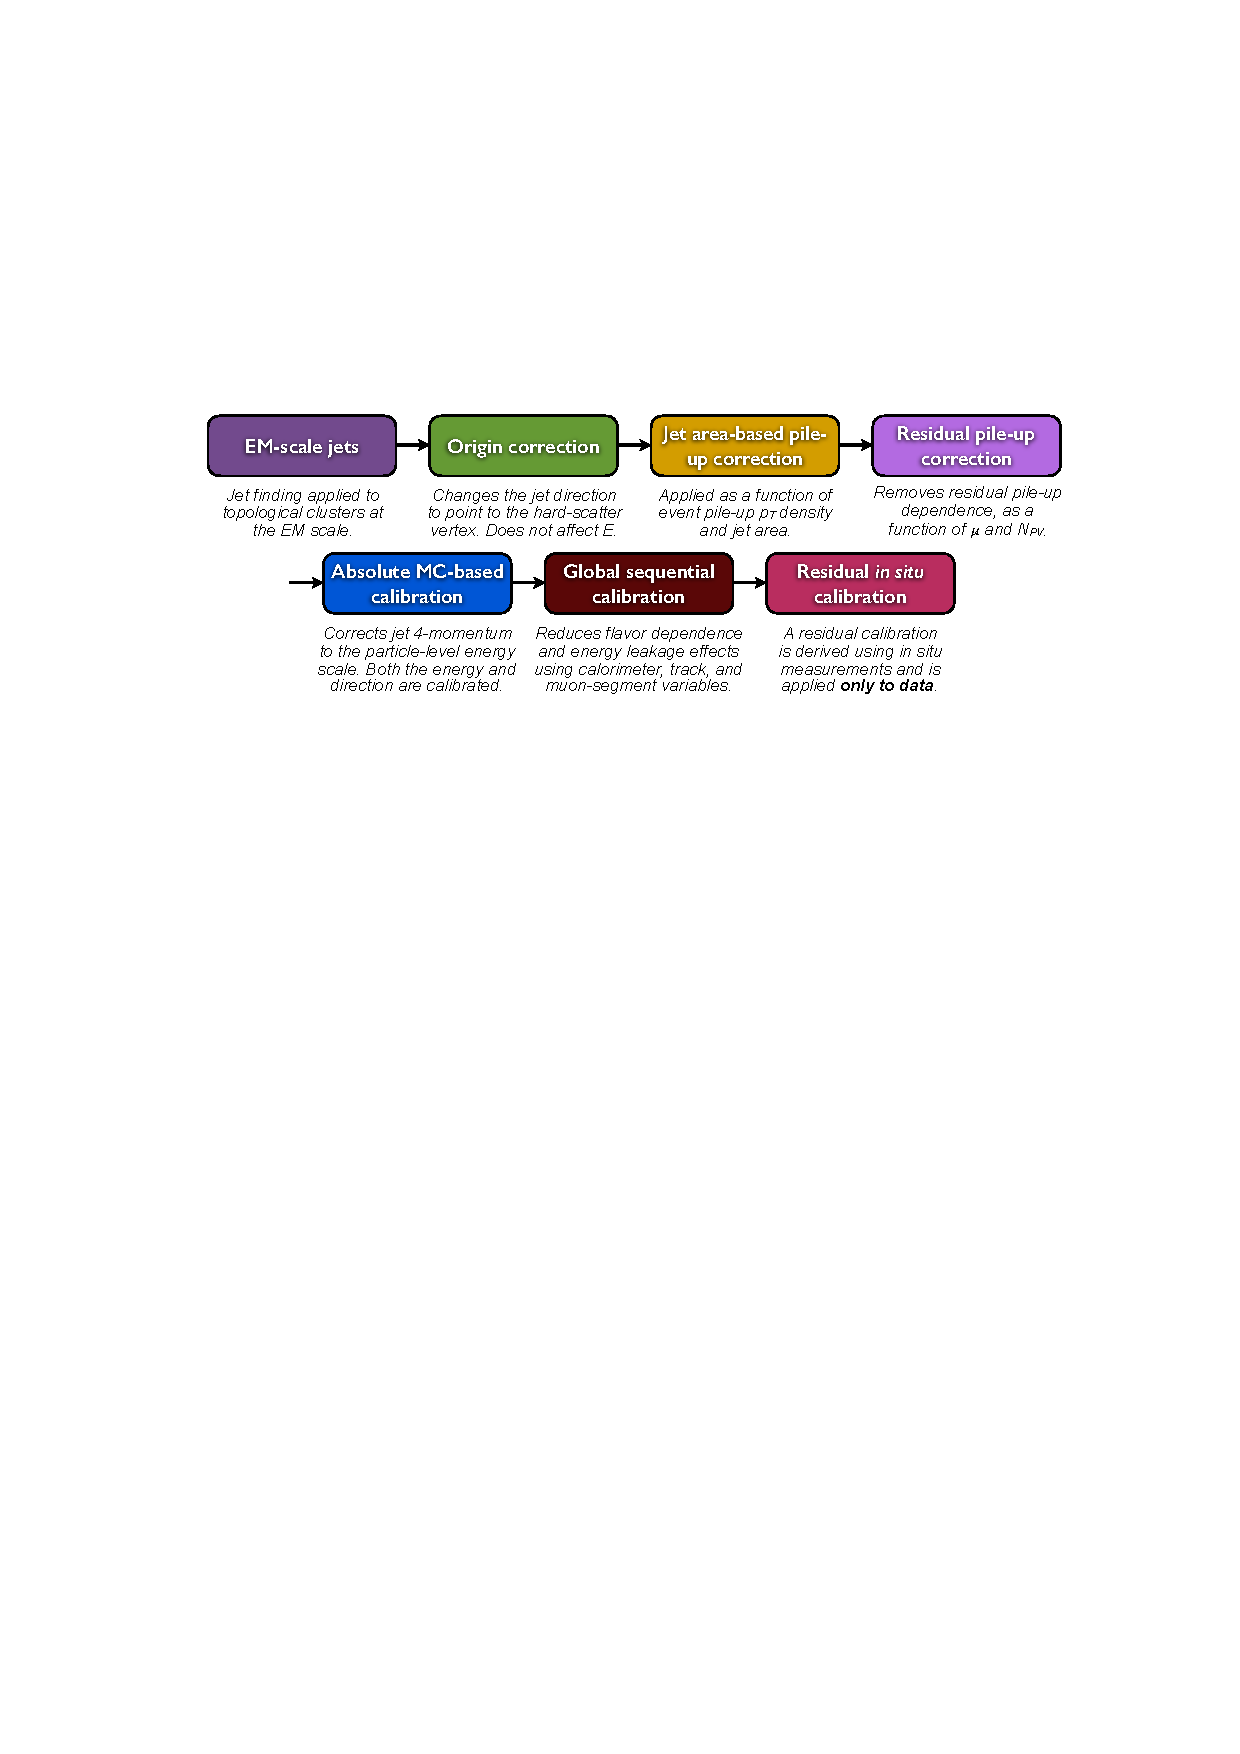
\includegraphics[width=0.9\textwidth]{figs/Objects/jets_calib_schem.pdf}
    \caption[Calibration stages for the EM+JES calibration scheme.]
            {Calibration stages for the EM+JES calibration scheme~\cite{obj-jets_calib_run2}.}
    \label{fig:obj-jets_calib_schem}
  \end{center}
  \vspace{-0.5cm}
\end{figure}

\noindent
To discuss each step in a little more detail:
\begin{itemize}[leftmargin=*]
\item\textbf{Origin Correction}:
  This step changes the direction of the jets such that the four-momentum points to the hard-scatter primary vertex
  rather than the centre of the detector.
  This calculation conserves the jet energy.\vspace{0.5em}
\item\textbf{Jet Area-Based Pile-up Correction}:
  This step removes unwanted energy contributions from pile-up.
  This correction subtracts the area of the jet, $A$, multiplied by the average energy density due to pile-up, $\rho$.\vspace{0.5em}
\item\textbf{Residual Pile-up Correction}:
  This step further reduces effects from pile-up utilising the linear dependence of pile-up effects on
  the number of primary vertices, $N_{PV}$
  and the mean number of additional $pp$ collisions per bunch crossing of the event, $\mu$.\vspace{0.5em}
\item\textbf{Absolute JES Correction}:
  This step corrects the jet four-momentum from the EM-scale, at which they were initially formed,
  to the hadronic-scale, which is defined in terms of the truth jets in simulation.
  This correction is derived using truth jets and reconstructed detector-level jets in dijet Monte-Carlo events.\vspace{0.5em}
\item\textbf{Global Sequential Calibration}:
  This step uses information from the calorimeter, muon spectrometer and track-based variables
  to refine the reconstructed energy and reduce the overall uncertainties.\vspace{0.5em}
\item\textbf{In-situ calibration}:
  All previous steps in this calibration have been done using simulation to correct
  detector-level jets to truth jets. This step accounts for any differences between simulation and data.
  This step uses events containing a jet to be calibrated and a well-measured reference objects, including photons, Z bosons, and calibrated jets.
  Then conservation of momentum gives us information on the true $p_T$ of the jet to be calibrated.
  One can calculate a double ratio with respect to jet-$p_T$;
  \begin{equation}
    \text{Correction} = \frac{1}{R(p_T, \eta)} = \frac{ < p_T^{\text{jet}}/p_T^{\text{ref}}>_{\text{MC}} }{ < p_T^{\text{jet}}/p_T^{\text{ref}}>_{\text{Data}} }
  \end{equation}
  which is applied as a correction to jet $p_T$ in data; this correction is not applied in simulation.
\end{itemize}

This calibration scheme is known as an EM+JES, as the topoclusters are at the EM-scale.
Here, I should note that there are other schemes used for calibrating jets at ATLAS,
for example some analyses~\cite{obj-VVjj} correct each topocluster to the hadronic scale
before clustering the jet, in a scheme called Local Cluster Weighted (LCW)~\cite{obj-jets_topo}.
EM+JES is generally used in ATLAS analyses as it is a simpler calibration scheme than LCW, but provides similar results.

The end result of the processes described in this section is a jet,
reconstructed from EM-scale topoclusters using an anti-$k_T$ algorithm with a jet width parameter $R$=0.4,
which has been calibrated using simulation and a data-driven in-situ step.
The result of this process is what is known as an anti-$k_T$ R=0.4 EM+JES jet,
and is the definition for a jet in this thesis.

\subsection{Jet Energy Uncertainties}
\label{sec:obj-jets_uncert}

All measurements have uncertainties, and this section investigates the uncertainties of jet energy measurement.
Jet energy measurements separate the associated uncertainties into two components;
jet energy resolution and jet energy scale.

Jet energy resolution (JER) is defined as $\sigma(E)/E$, and JER uncertainties
come from an imperfect simulation of detector resolution in Monte-Carlo simulation.
This uncertainty is measured using an in-situ technique from the balancing of jets in 8 TeV collision data
which is extrapolated for 13 TeV data; the final uncertainty accounts for this extrapolation.
Figure~\ref{fig:obj-jets_calib_JER} shows the fractional JER uncertainty as a function of jet-$p_T$ and jet-$\eta$.
Full details on the derivation of this uncertainty can be found in~\cite{obj-jets_calib_2015}~and~\cite{obj-jets_calib_JER_8TeV}.

\begin{figure}[!ht]
  \begin{center}
    \captionsetup[subfigure]{aboveskip=0pt,justification=centering}
    \subcaptionbox{Jet-\pT} {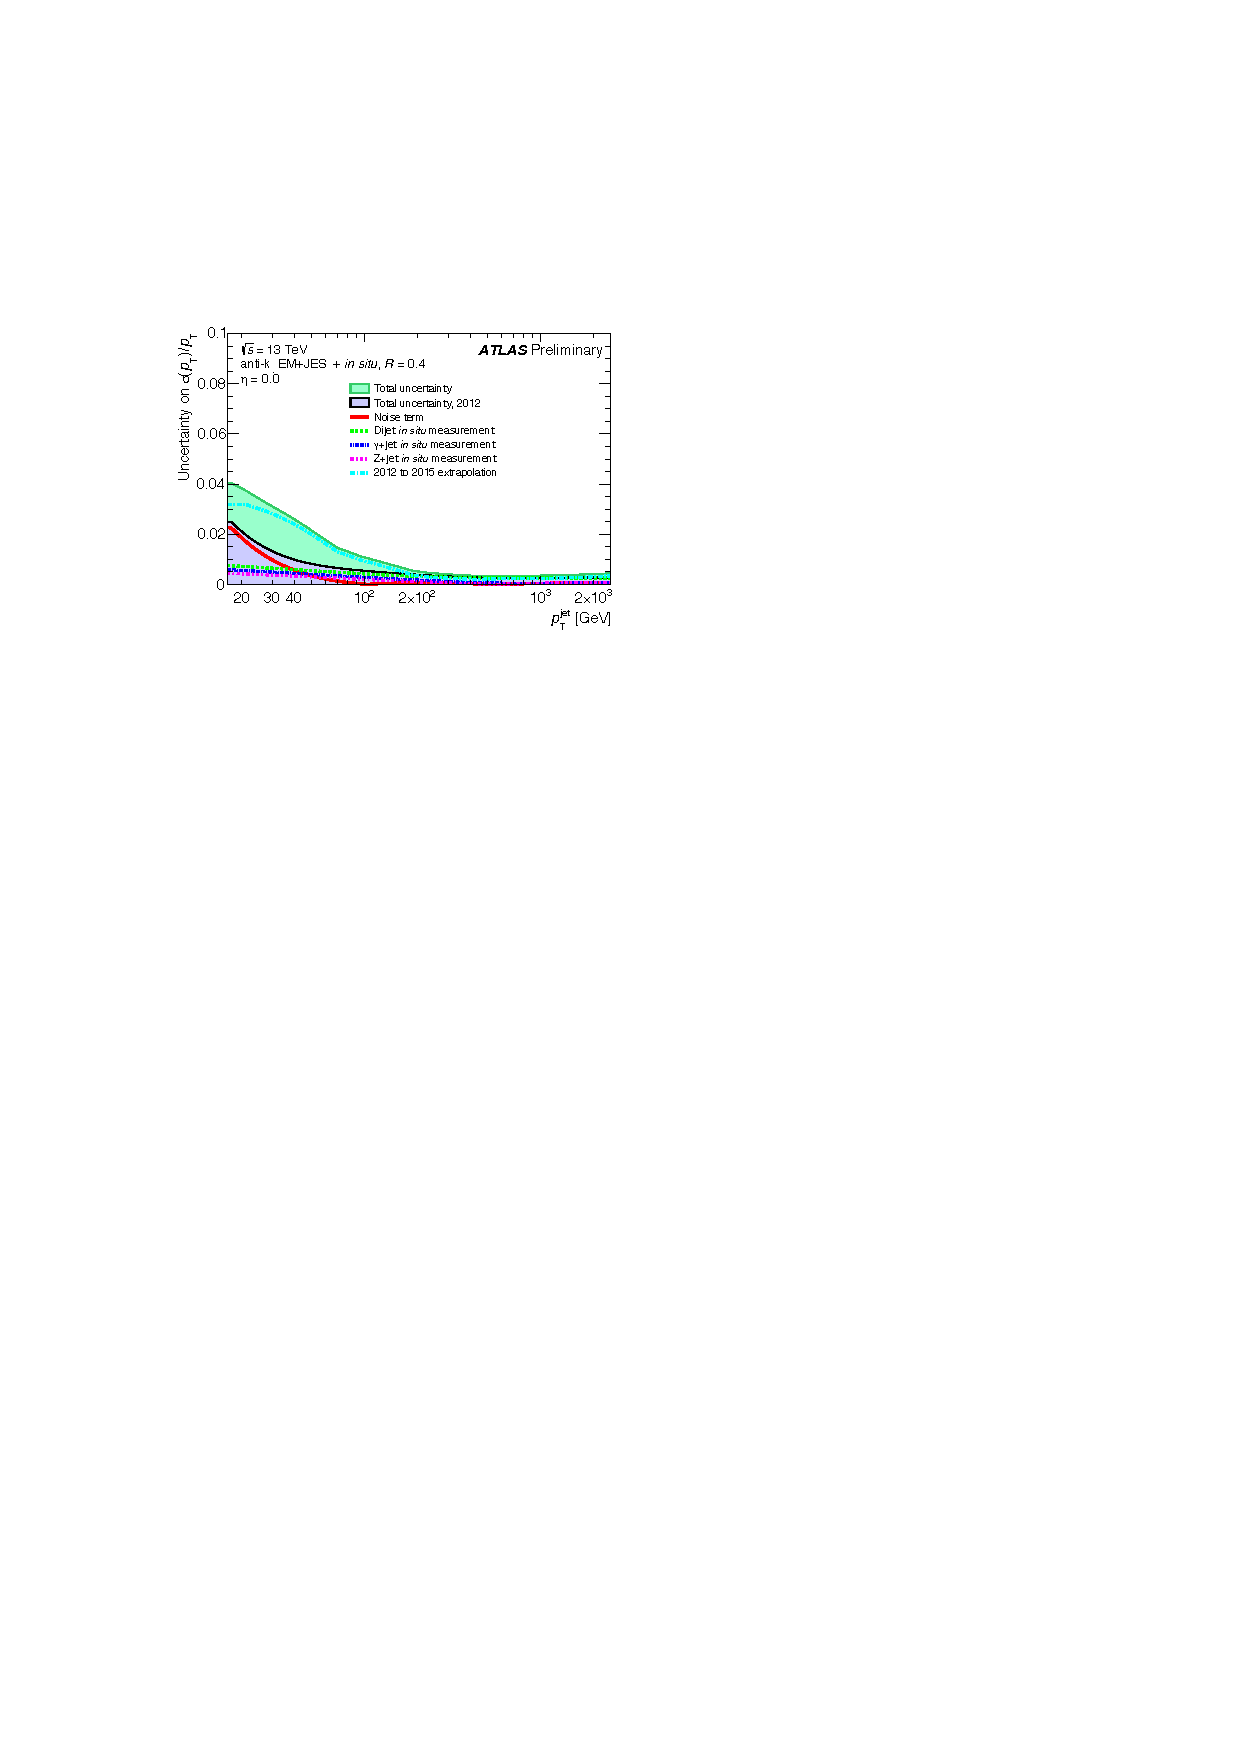
\includegraphics[width=0.45\linewidth, angle=0]{figs/Objects/jets_uncert_JER_pt.pdf} }
    \subcaptionbox{Jet-\eta}{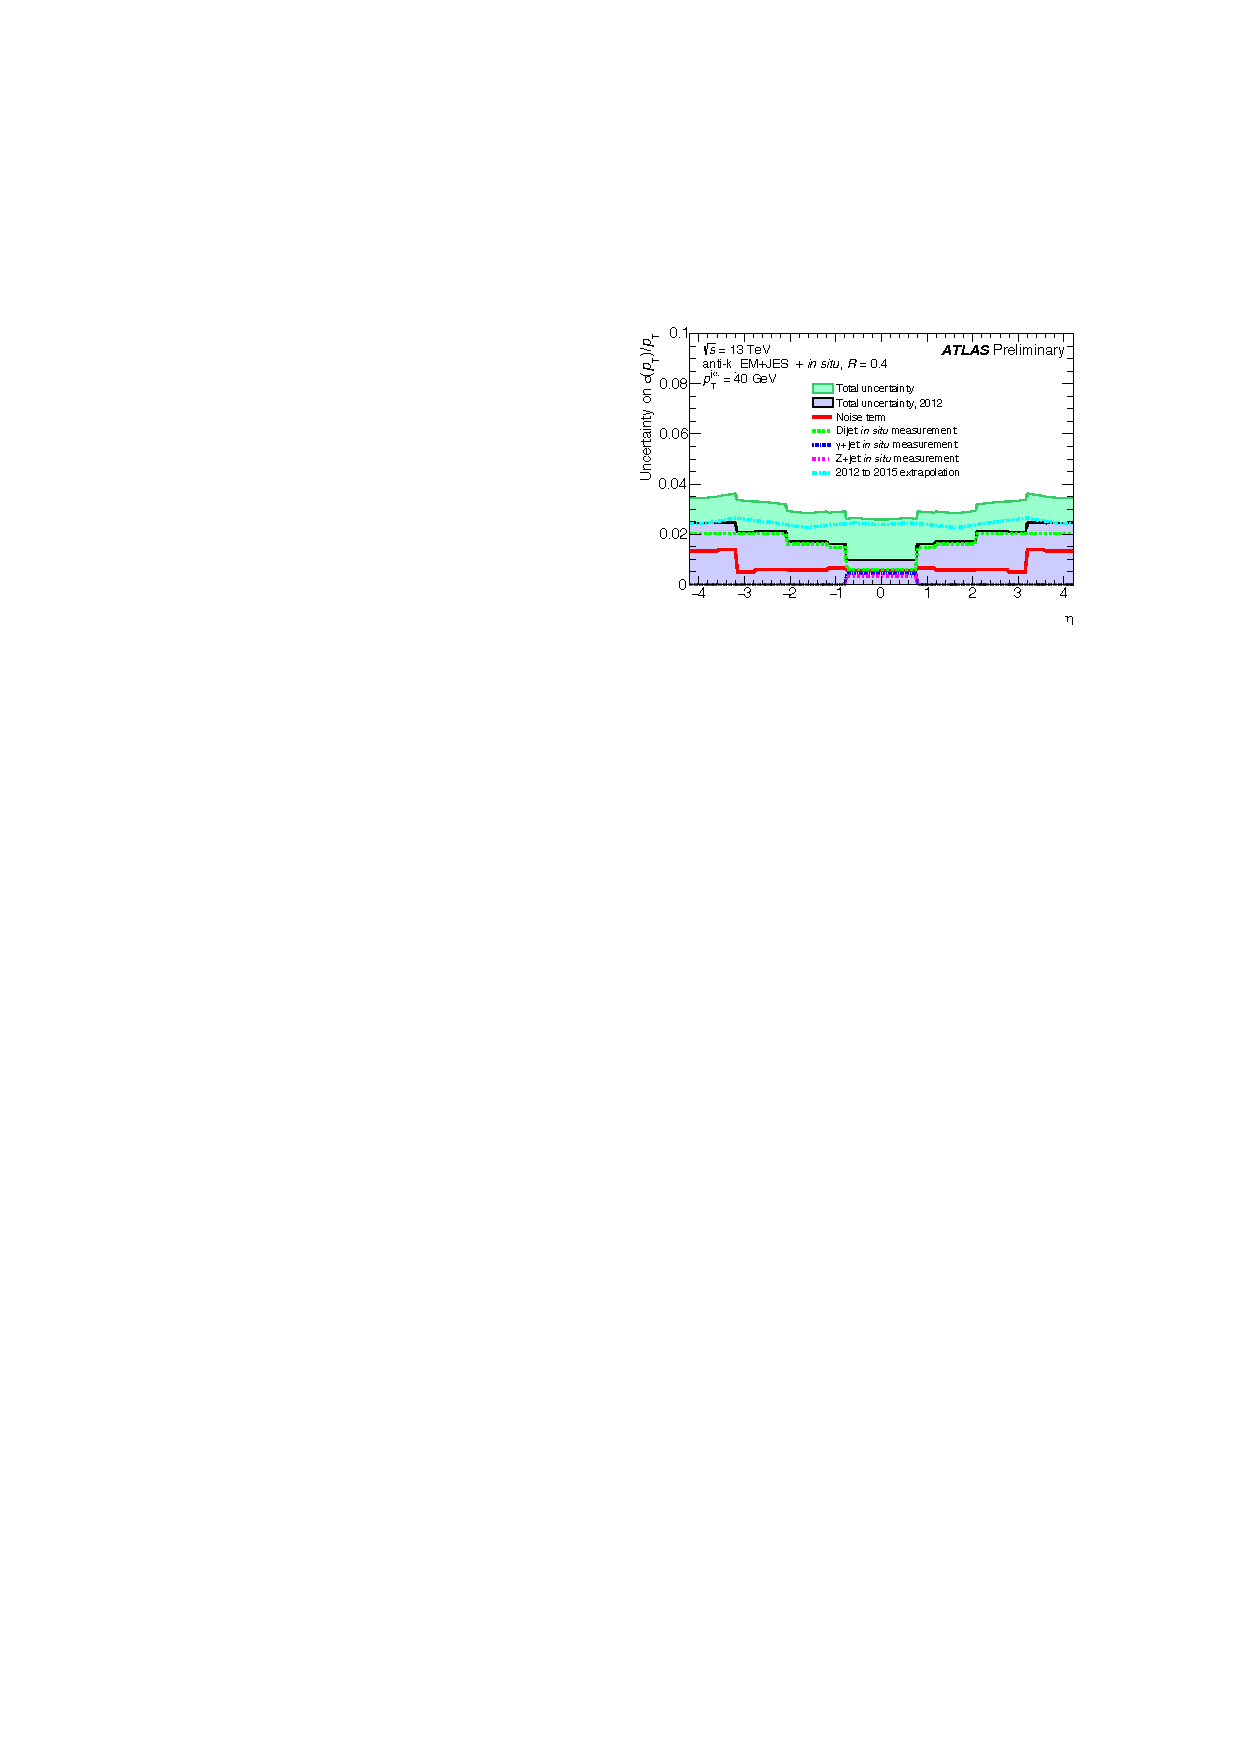
\includegraphics[width=0.45\linewidth, angle=0]{figs/Objects/jets_uncert_JER_eta.pdf} }
  \end{center}
  \caption[The fractional jet energy resolution uncertainty as a function of jet-\pT and \eta.
    The total uncertainty is shown as are the contributions from the various sources of uncertainty.]
          {The fractional jet energy resolution uncertainty as a function of jet-\pT and \eta.
            The total uncertainty is shown as are the contributions from the various sources of uncertainty ~\cite{obj-jets_calib_2015}.}
  \label{fig:obj-jets_calib_JER}
\end{figure}
\FloatBarrier
Jet energy scale (JES) uncertainties arise from the calibration procedure
to correct jets from the EM-scale to the hadronic-scale, outline above.
80 separate uncertainties are derived to cover each step of the calibration,
the dominant uncertainties arise from the data-driven in-situ step~\cite{obj-jets_calib_run2}.
Figure~\ref{fig:obj-jets_calib_JES} shows the fractional JES uncertainty as a function of jet-$p_T$ and jet-$\eta$.

\begin{figure}[!ht]
  \begin{center}
    \captionsetup[subfigure]{aboveskip=0pt,justification=centering}
    \subcaptionbox{Jet-\pT} {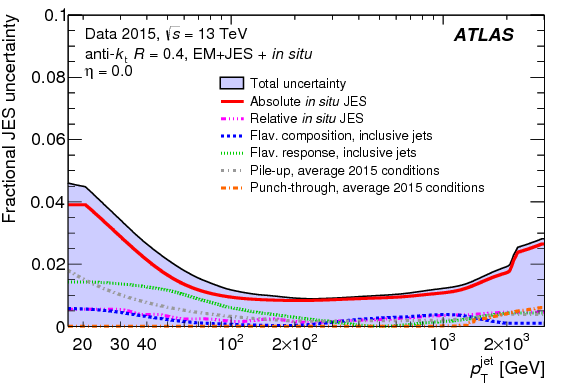
\includegraphics[width=0.45\linewidth, angle=0]{figs/Objects/jets_uncert_JES_pt.png} }
    \subcaptionbox{Jet-\eta}{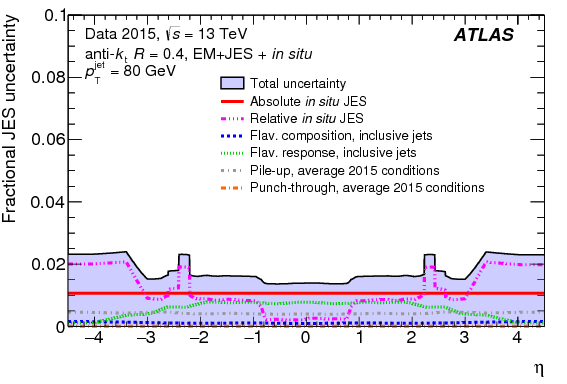
\includegraphics[width=0.45\linewidth, angle=0]{figs/Objects/jets_uncert_JES_eta.png} }
  \end{center}
  \caption[The fractional jet energy scale uncertainty as a function of jet-\pT and \eta.
    The total uncertainty is shown as are the contributions from the various sources of uncertainty.]
          {The fractional jet energy scale uncertainty as a function of jet-\pT and \eta.
            The total uncertainty is shown as are the contributions from the various sources of uncertainty ~\cite{obj-jets_calib_run2}.}
  \label{fig:obj-jets_calib_JES}
\end{figure}

\FloatBarrier

\newpage
\section{$b$-Jets}
\label{sec:obj-bjets}

Hadronic jets, described in Section~\ref{sec:obj-jets}, can be further categorised into three separate categories based on the flavour of the constituent quarks.
$b$-jets are defined as jets containing one or more $b$-hadrons,
$c$-jets are defined as jets containing one or more $c$-hadrons but no $b$-hadrons
and finally light-flavoured jets comprise of only light hadrons (formed of $u$, $d$ and $s$ quarks).
A description of how this definition is practically used in simulation is given in Section~\ref{sec:obj-bjets_label}.

The identification of $b$-jets, known as $b$-tagging, is an essential tool in a range of ATLAS collaboration results;
for example analyses studying the $t\bar{t}$ final state \cite{obj-ttbar}
\footnote{Section~\ref{sec:trig-bjet_eff} contains an analysis utilising $b$-tagging in the $t\bar{t}$ final state.}
and the first direct evidence of the Higgs boson coupling to the quark-sector~\cite{obj-Hbb}.
%In the former, as the top decays to a \textit{W}-boson and a $b$-quark with a branching ratio close to 100\%, 
%the application of $b$-tagging can be used increase purity, this is used in the study described in Section~\ref{sec:trig-sys}.
%In the latter, the Higgs boson coupling is proportional to mass squared, hence the large mass of the
%$b$-quark means that $H\to b\bar{b}$ is the decay of the Higgs boson with the largest branching-ratio
%which means that it is the best channel to make the first direct observation of the Higgs boson coupling to fermions.
In the same sense, identification of $b$-jets is an essential part of the analysis being presented here;
by selecting $b$-jets we increase our sensitivity to BSM models that decay to 1 or 2 $b$-jets in their final state.
\textbf{LM Fix, link to where I explain why this is good, maybe Intro}.

The process of $b$-tagging at ATLAS in Run-2 has been previously described in great
detail~\cite{obj-bjets_algo_2015,obj-bjets_algo_2016},
so what follows is a summary of the key features of the process.

\subsection{Assigning a Flavour Label}
\label{sec:obj-bjets_label}

In simulation, the particle-level truth information is known, and hence a truth flavour label of a jet can be defined.
Flavour is assigned to jets by matching truth-level heavy-hadrons with $p_{T} >$ 5 GeV and $\Delta R <$ 0.3 between the hadron and the jet.
If a $b$-hadron is matched to a jet, the jet is then declared a $b$-jet;
this process is then repeated for $c$-hadrons and then $\tau$ leptons.
If no match between $b$, $c$ or $\tau$ is achieved then the jet is assigned as a light-flavour jet.
The matching is exclusive, which means that each particle is only assigned to one jet.
This definition of truth flavour in simulation is used generally within this thesis.
   
\subsection{Baseline $b$-tagging Algorithms}

To identify $b$-jets, $b$-tagging algorithms utilise the long lifetimes of the heavy-hadrons that decay through the flavour changing weak interaction.
A hadron containing a $b$-quark has a lifetime $\sim$\SI{1.6}{\pico\second} ~\cite{obj-bjets_PDG}.
%Note to laurie - First year talk contains this calc
%   p = gamma m v
%   d = vt = v gamma tau
%   d = p tau / m
%   Plug in numbers.
A $b$-jet decay chain  will typically contain two of these flavour changing interactions, 
as at the quark level, the $b$-quark contained in the jet will decay to a $c$-quark, which will then decay into a $u$ or $d$ quark.
The lifetimes of the heavy flavour hadrons means that they will decay a measurable distance from the 
primary vertex, the point where the hard-scatter collision occurs;
for example a $B_0$ meson with a $p_T$ of $x$ GeV will travel approximately $x/10$ mm.
Hence, the flavour of a jet can be inferred from the presence of particles
that originate from a point offset from the primary vertex.

In practice this is performed using the topology of tracks and properties of the jets,
which have been described in Section~\ref{sec:obj-tracks} and \ref{sec:obj-jets} respectively.
To utilise tracks and jets in tandem one must associate the tracks to the jets,
which is performed by requiring small angular separation $\Delta R$ between the two objects.
The maximum value of $\Delta R$ for association varies as a function of the jet-$p_T$,
resulting in a narrower cone for high-$p_T$ jets which are more collimated.
At 20 GeV, it is 0.45 while for more energetic jets with a pT of 150 GeV the cut is 0.26.
Tracks are exclusively matched, meaning each track is only associated with one jet, chosen using the smallest value of $\Delta R$.

There are three base $b$-tagging algorithms utilised to produce discriminating variables \cite{obj-bjets_algo_2016}, which are described in the next three sections.
%Sections~\ref{sec:obj-bjets_IP}~to~\ref{sec:obj-bjets_JF}.
The variables are then combined in a multi-variate algorithm which is described in Section~\ref{sec:obj-bjets_MV2}.
Figure~\ref{fig:obj_bjets_schem} shows a schematic illustrating how tracks
are used by the three $b$-tagging algorithms to identify a $b$-jet,
the details of this figure are referred to in the following three sections.

\begin{figure}[!htb]
  \begin{center}
    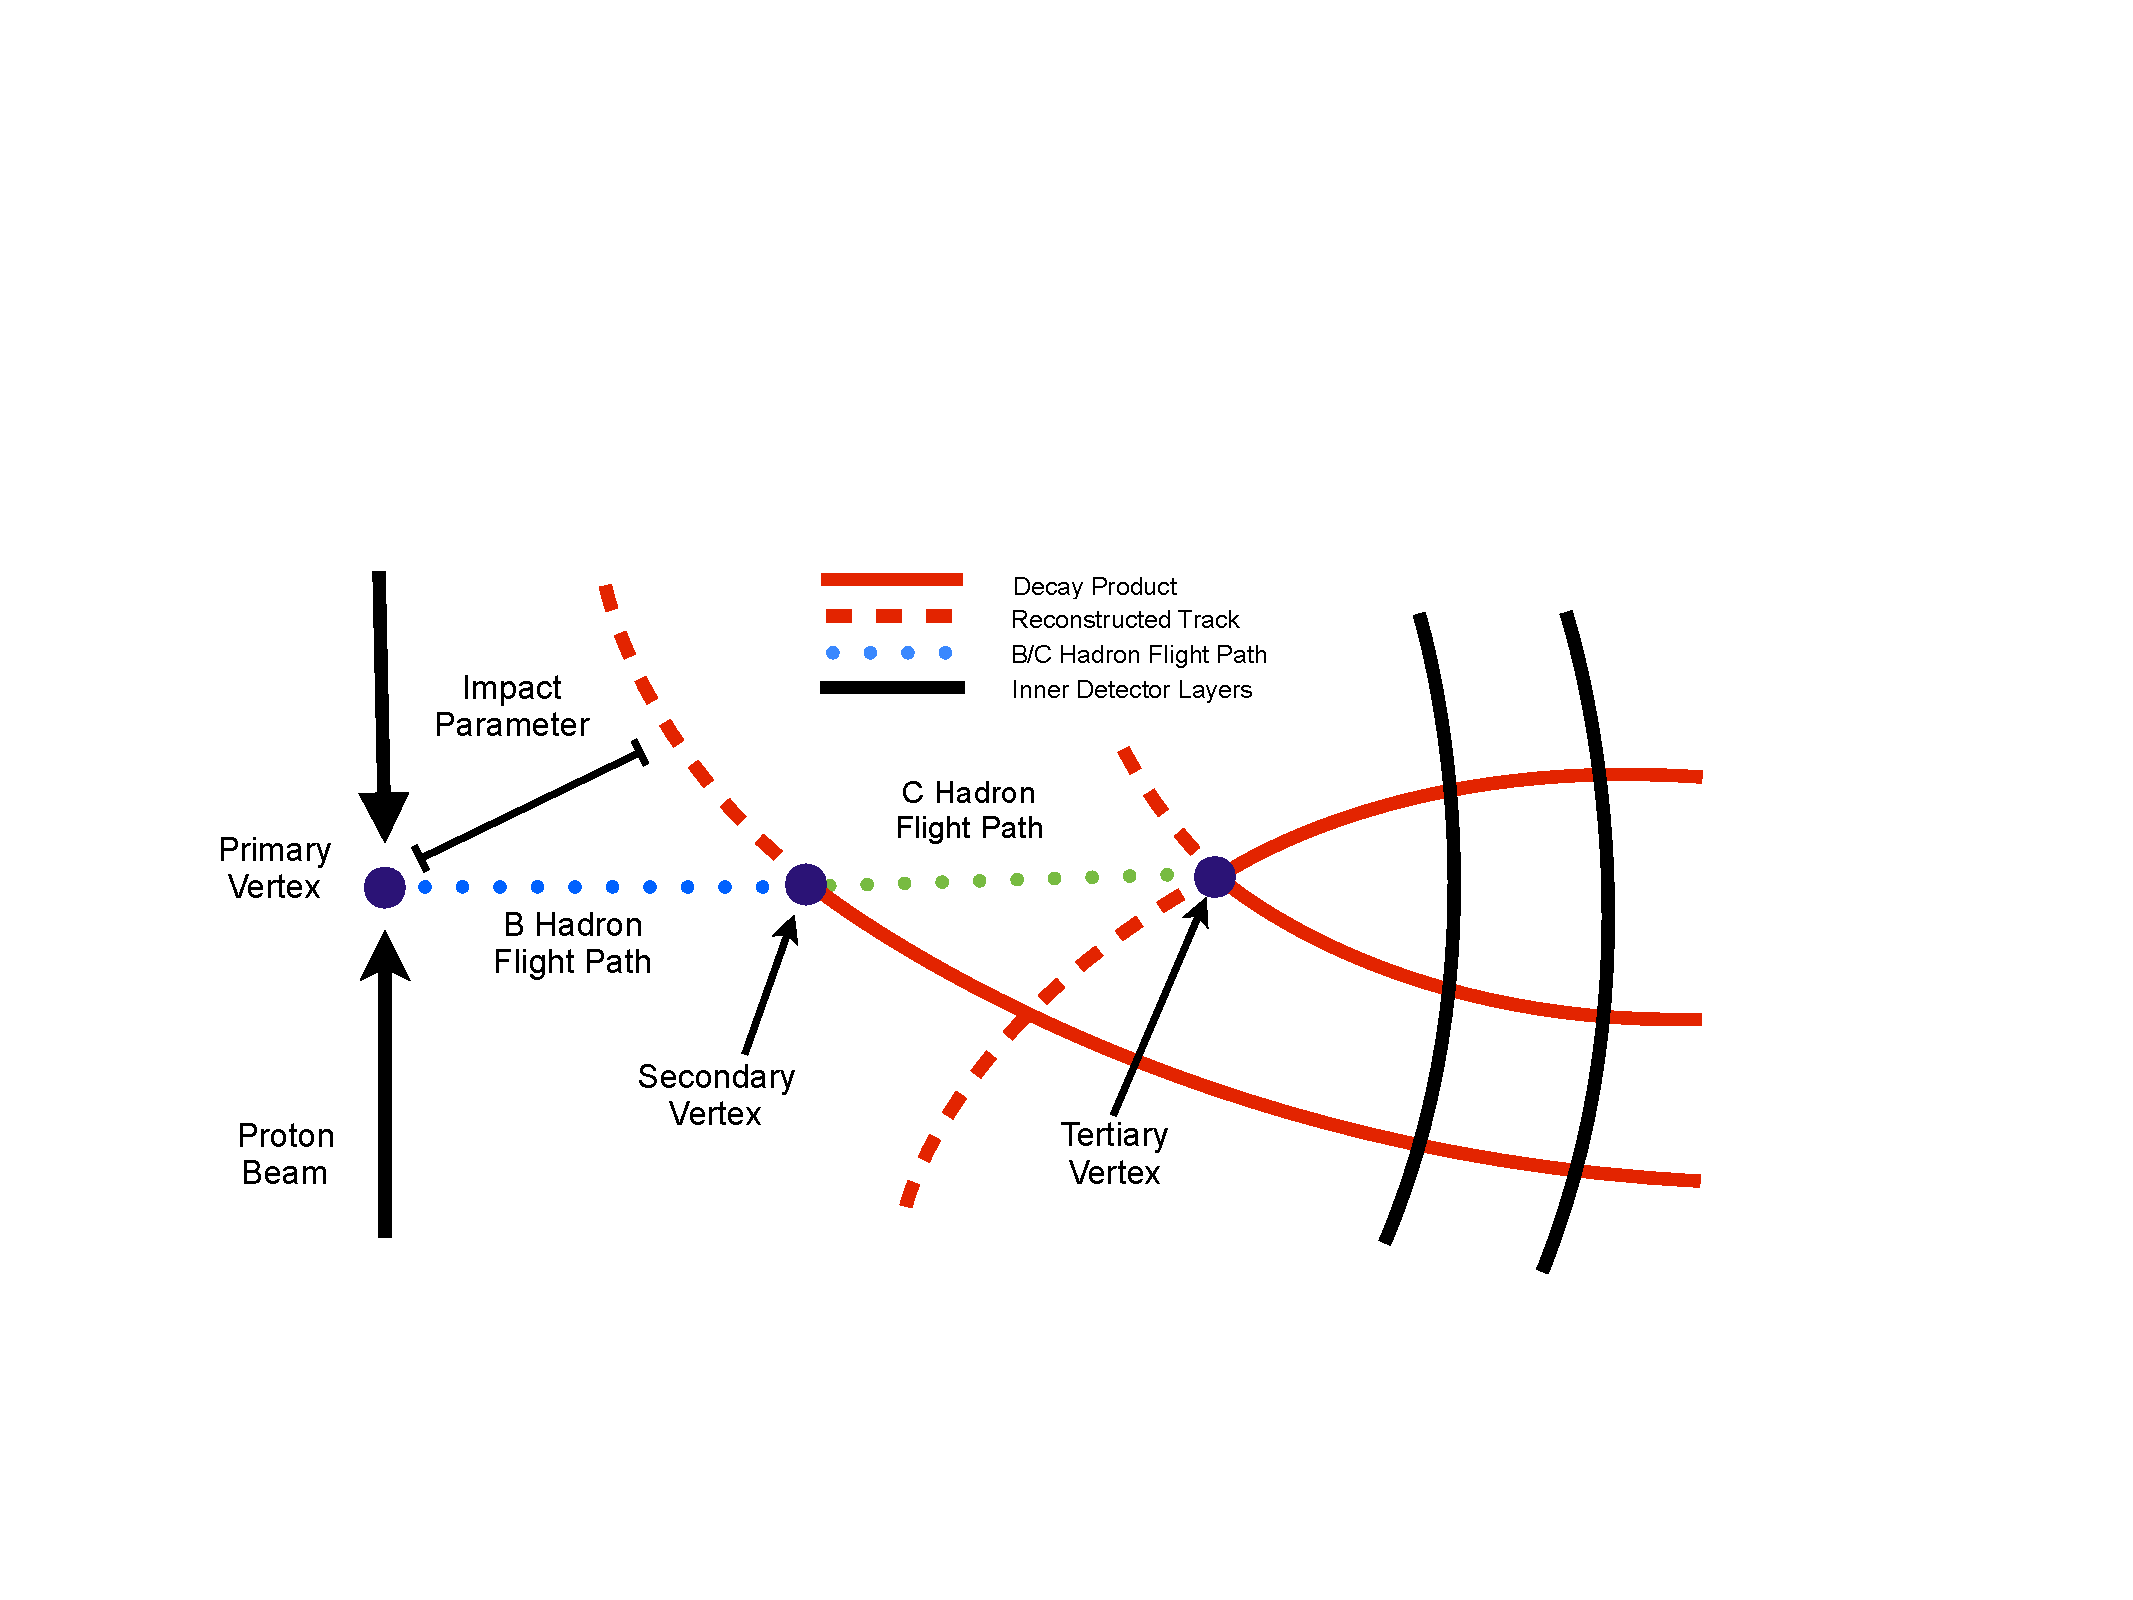
\includegraphics[width=0.9\textwidth]{figs/Objects/bjets_schem.pdf}
    \caption{A diagram to illustrate the key features of a $b$-jet that are utilised by the base $b$-tagging algorithms.}
    \label{fig:obj_bjets_schem}
  \end{center}
  \vspace{-0.5cm}
\end{figure}

\subsubsection{Impact parameter based}
\label{sec:obj-bjets_IP}

The IP3D algorithm is utilises the impact parameter, which is defined as the shortest distance between a specific track and the primary vertex.
A track corresponding to a particle coming from the offset decay vertex of a heavy-hadron is likely to have a large impact parameter,
meaning that the distribution of track impact parameter is different for each of the jet-flavours.
The impact parameter of a track coming from the decay of a heavy hadron is indicated in Figure~\ref{fig:obj_bjets_schem}.
In this algorithm, for all tracks associated to a jet, the impact parameter is calculated in both the transverse (perpendicular to beam-line)
and longitudinal (parallel to beam-line) direction, which are referred to as $d_{0}$ and $z_{0}$.
Then the IP3D algorithm calculates a likelihood of the jet having a specific flavour, 
based on the distributions of the impact parameters ($d_{0}$, $z_{0}$) and their significances 
($d_{0}/\sigma _{d0}$ and  $z_{0}/\sigma_{z0}$) for tracks within the jet. 
Another similar algorithm, IP2D, also calculates the jet flavour likelihood from just the transverse distributions, ($d_{0}$ and $d_{0}$ significance), which is more
robust to pile-up, as tracks from pile-up jets are likely to have a large $z_{0}$ significance value.

\subsubsection{Secondary vertex}
\label{sec:obj-bjets_SV}


The SV1 algorithm aims to reconstruct a secondary vertex of two or more intersecting tracks, corresponding to the decay of a heavy-flavour hadron;
the secondary vertex within a $b$-jet's decay chain is illustrated in Figure~\ref{fig:obj_bjets_schem}.
The SV1 algorithm then calculates many variables that are associated with properties of the reconstructed secondary vertex that show flavour discrimination;
some example variables are the vertex invariant mass,
which will be larger for $b$-jets due to the heavy mass of the $b$-hadron
\footnote{Mass of a $B_0$-meson $\sim$ 5 GeV which is the most common $B$-hadron in a $b$-jet~\cite{obj-bjets_PDG}.}, 
the distance in the transverse plane between the primary vertex and the secondary vertex, % (2D flight path $L_{XY}$),
which will be larger for $b$-jets due to the long lifetime of the $b$-hadron,
and the number of tracks at the secondary vertex, which will be larger for reliable secondary vertices.

\subsubsection{Jet Fitter}
\label{sec:obj-bjets_JF}

The JetFitter algorithm (JF) attempts to reconstruct the full decay chain of the $b$-hadron into a charmed-hadron and then into light-hadrons. 
This is done by assuming that all vertices lie on a common $b$-flight axis, and then constructing vertices from the intersection of
one or more tracks and the flight axis.
The aim of this is to reconstruct the secondary and tertiary vertices which correspond to the decays of the $b$-hadron and charmed-hadron,
as illustrated in Figure \ref{fig:obj_bjets_schem}.
Similar to SV1, the JetFitter algorithm then calculates a number of flavour discriminating variables:
for example vertex mass and number of vertices with two or more tracks.

\subsection{Multi-Variate $b$-tagging Algorithm}
\label{sec:obj-bjets_MV2}

The three base algorithms are combined in a boosted decision tree (BDT), a machine-learning technique for combining the many flavour-discriminating variables,
resulting in an algorithm that is known as MV2.
As shown in Figure \ref{fig:obj-MV2_schem}, MV2 combines the likelihood output of IP3D and IP2D
with the discriminating variables of SV1 and JF discussed in the preceding sections,
resulting in an output between -1 and 1, where 1 indicates that the jet is very likely to be a $b$-jet and -1 indicates the inverse.

\begin{figure}[!htb]
  \begin{center}
    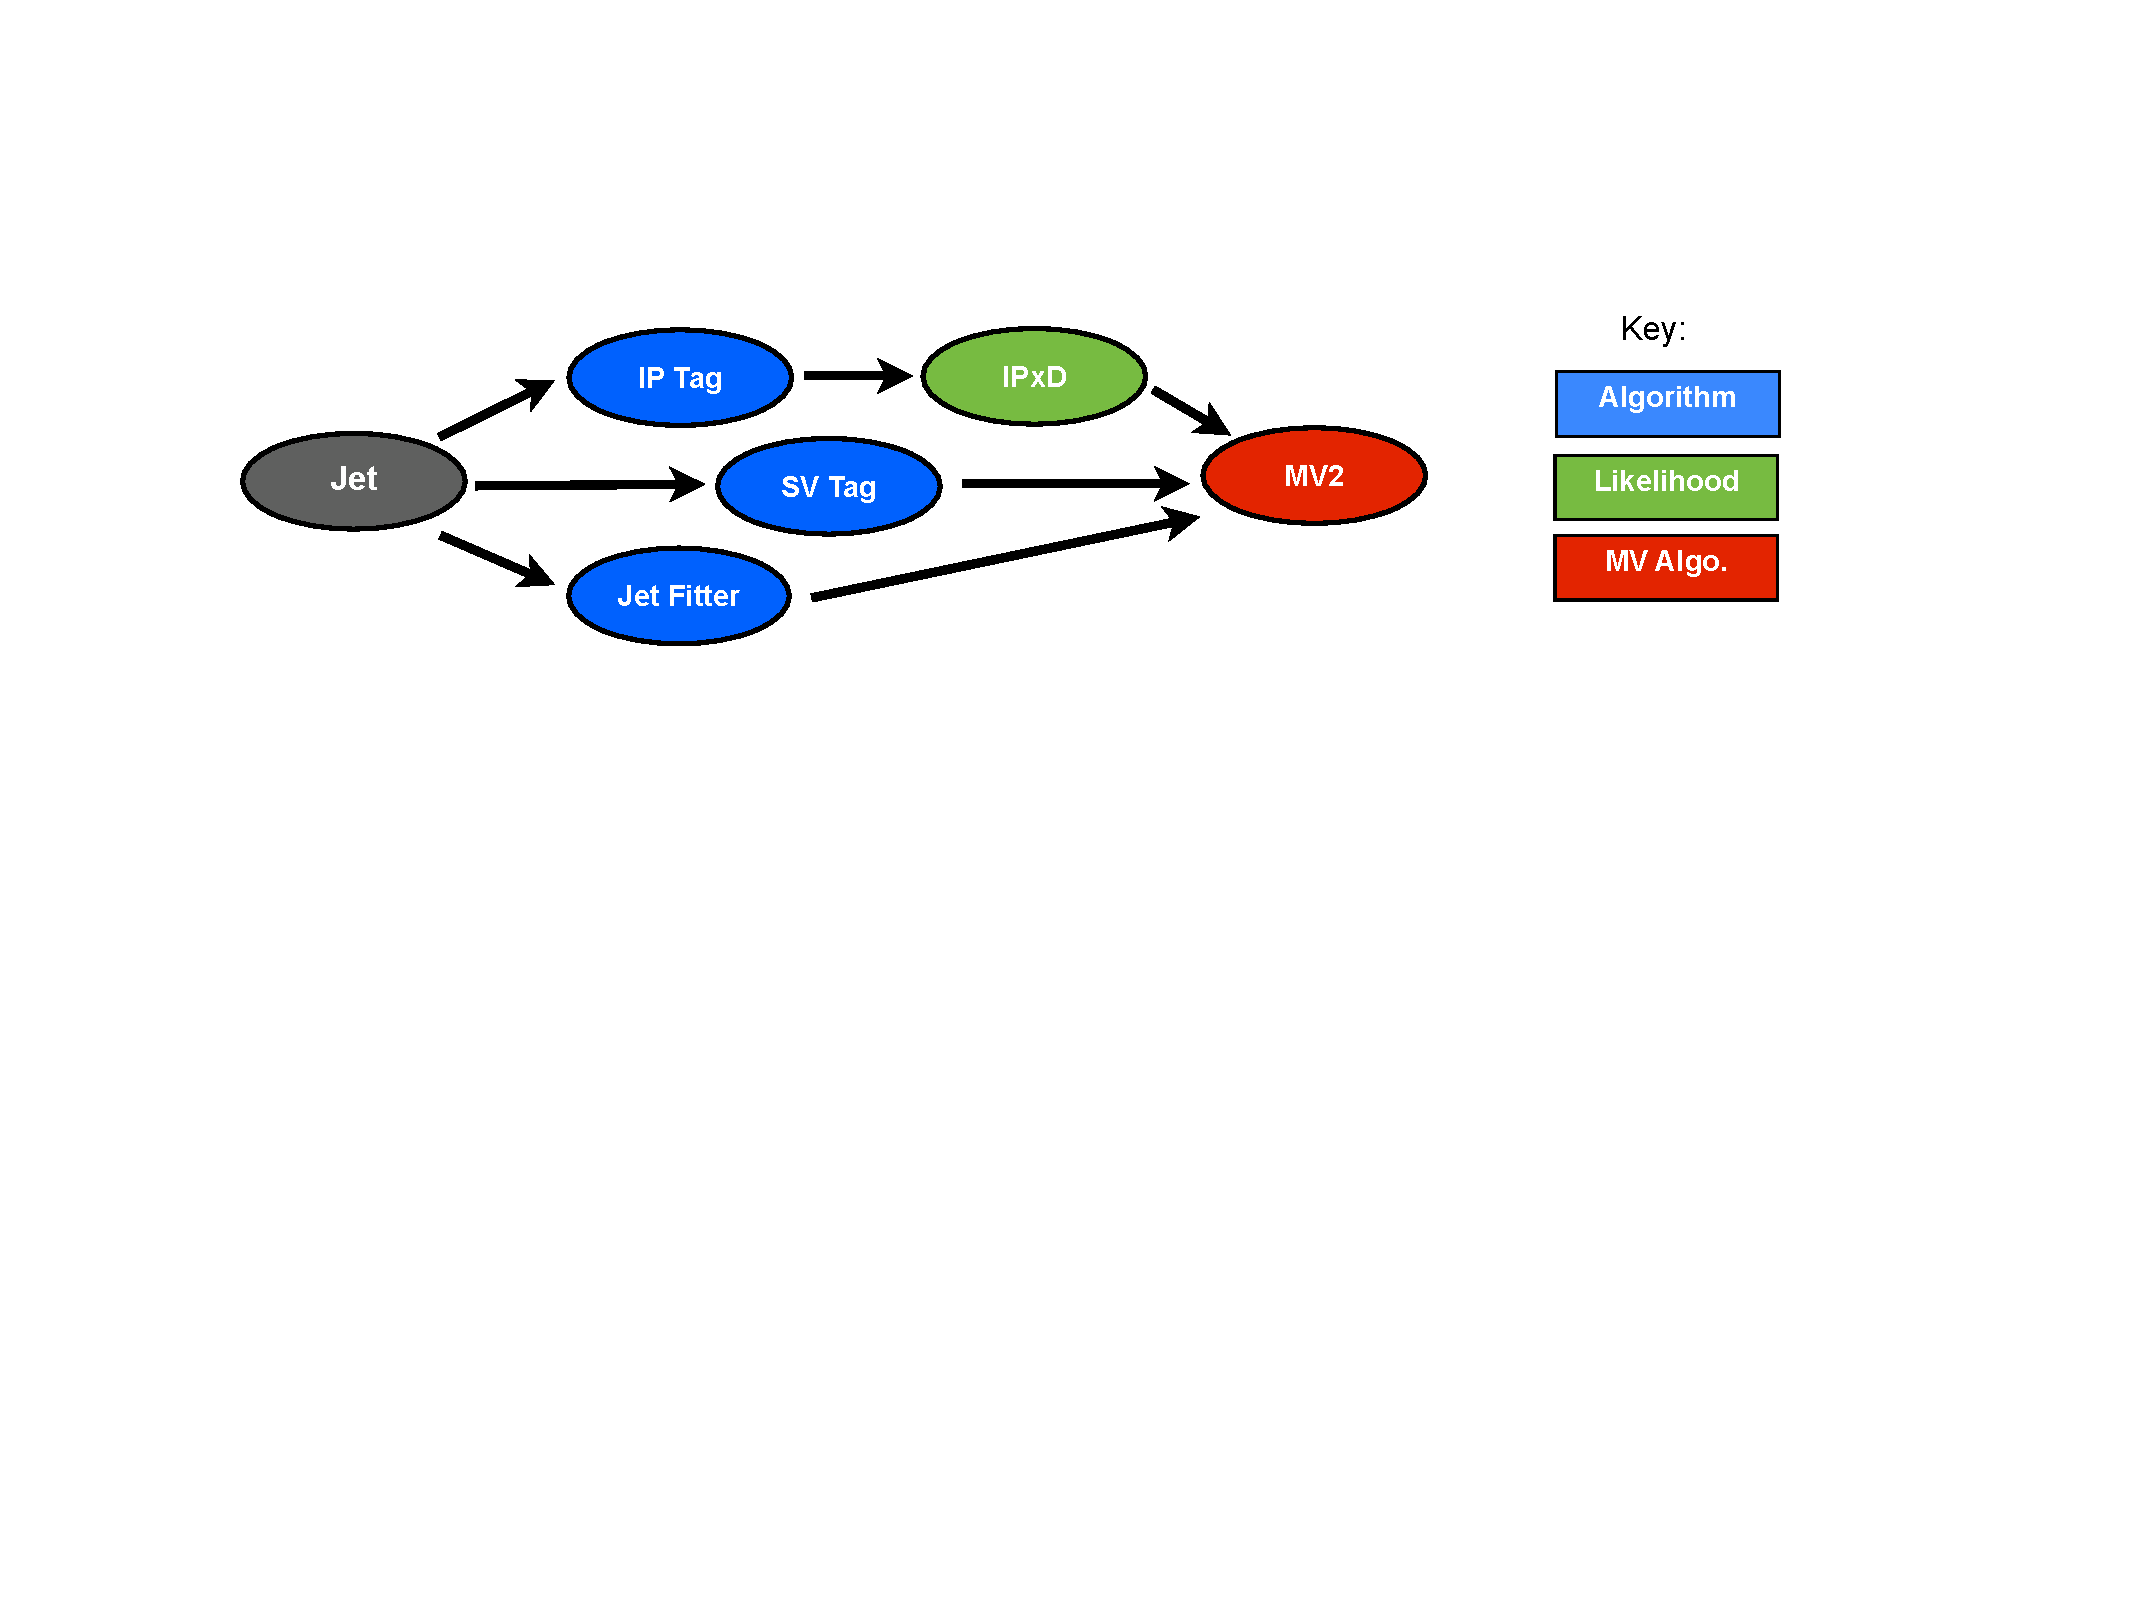
\includegraphics[width=1.0\textwidth]{figs/Objects/MV2_schem.pdf}
    \caption{A diagram illustrating how three base flavour tagging algorithms are combined in the MV2 algorithm.}
    \label{fig:obj-MV2_schem}
  \end{center}
  \vspace{-1cm}
\end{figure}


The BDT is trained using a simulated sample of $t\bar{t}$ events that will contain a mix of  $b$-, $c$- and light-jets
as well as a sample containing a $Z'$ boson decaying to $b$-quarks to increase statistics in the high jet-$p_T$ region.
The training makes use of the truth flavour labels assigned to jets using the process described in Section~\ref{sec:obj-bjets_label}.
A training sample with known truth labels is required as this allows the BDT to be optimised
such that it uses the complex correlations between the input variables to allow for high $b$-jet efficiencies
whilst still obtaining a large $c$- and light-jet rejection.
Subtly different algorithms can be obtained using samples containing different fractions of light and $c$-jets,
the fraction of $c$-jets used is labelled in the algorithm name;
for example the MV2c10 algorithm has been trained on a sample containing 10\% charm-jets, which gives strong light- and $c$-rejection.

A cut is then applied to this MV2 output in order to select jets that are likely to $b$-jets.
The choice of cut will vary the $b$-jet efficiency, light-jet rejection and $c$-jet rejection,
where $b$-jet efficiency is defined as the probability of accepting a true $b$-jet,
light-jet rejection is defined as 1 divided by the probability of accepting a true light-jet, and a similar definition applies for $c$-jet rejection.
Figure~\ref{fig:obj-bjets_perf} shows the $b$-jet efficiency against (a) light and (b) $c$-jet rejection of the MV2 algorithm for a continuous range of cuts.
The different lines show the performance of the algorithm in the 2015 configuration~\cite{obj-bjets_algo_2015}
and in the 2016 configuration~\cite{obj-bjets_algo_2016} where a range of different fraction of $c$-jets are used in the training;
2016 MV2c10 is the configuration used generally in this thesis as recommended in~\cite{obj-bjets_algo_2016}.
    
\begin{figure}[!ht]
  \begin{center}
    \captionsetup[subfigure]{aboveskip=0pt,justification=centering}
    \subcaptionbox{} {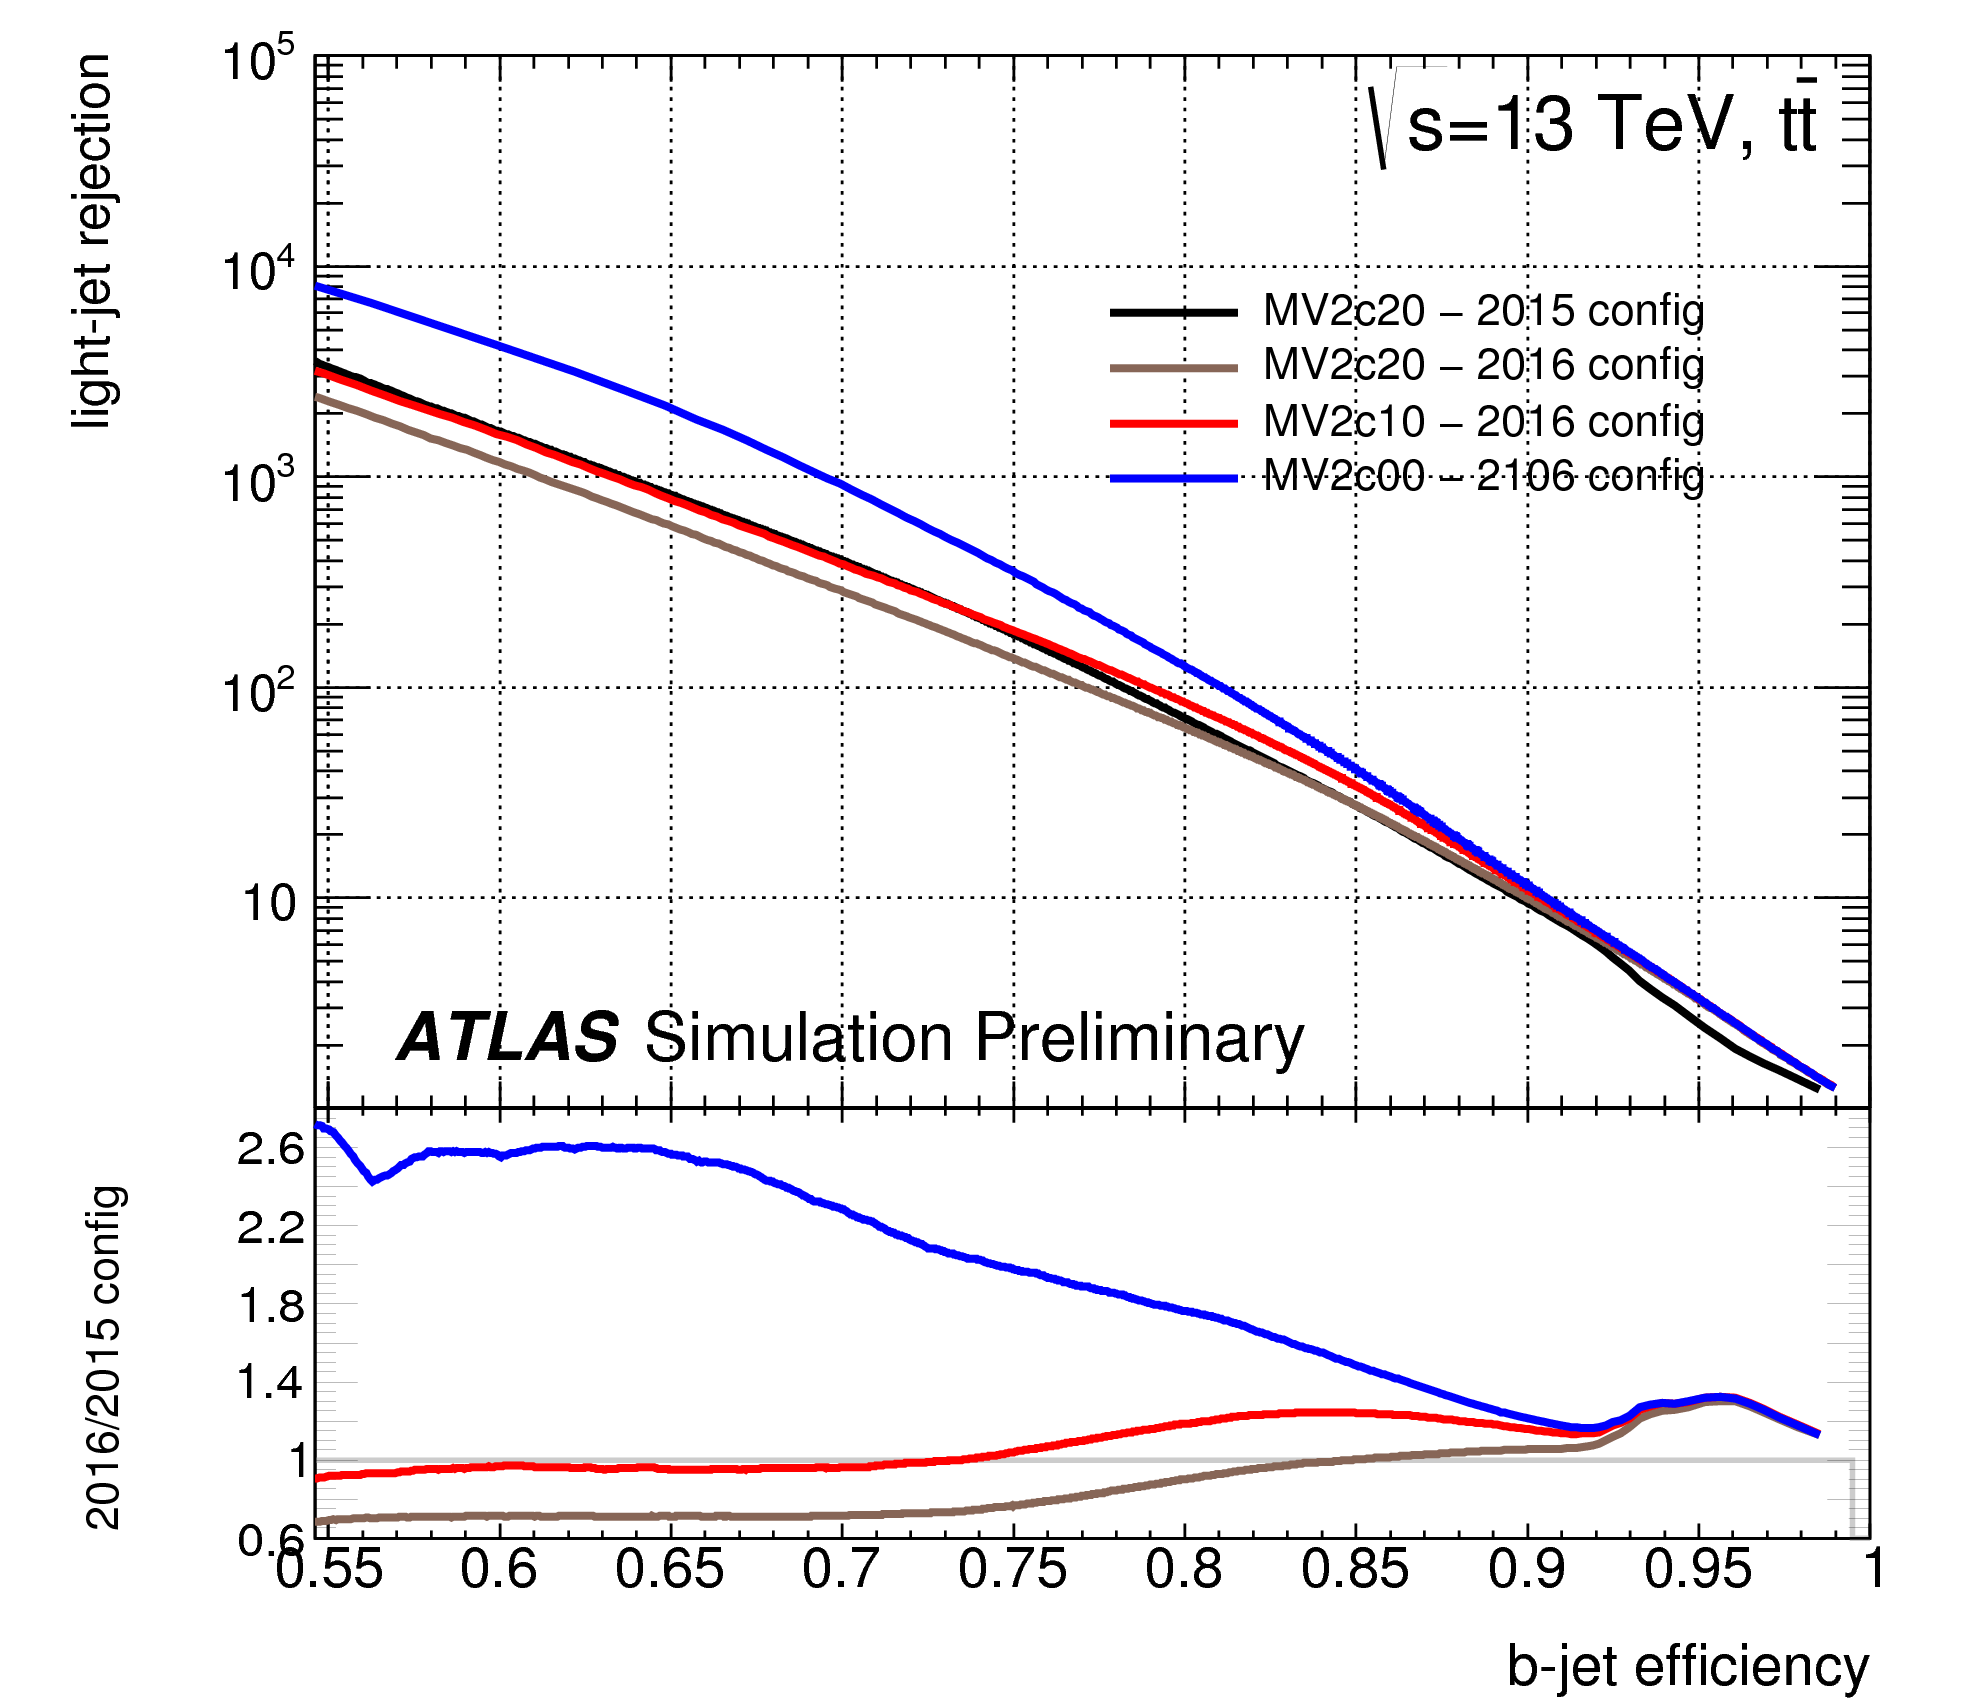
\includegraphics[width=0.48\linewidth, angle=0]{figs/Objects/bjets_perf_light}}
    \subcaptionbox{} { 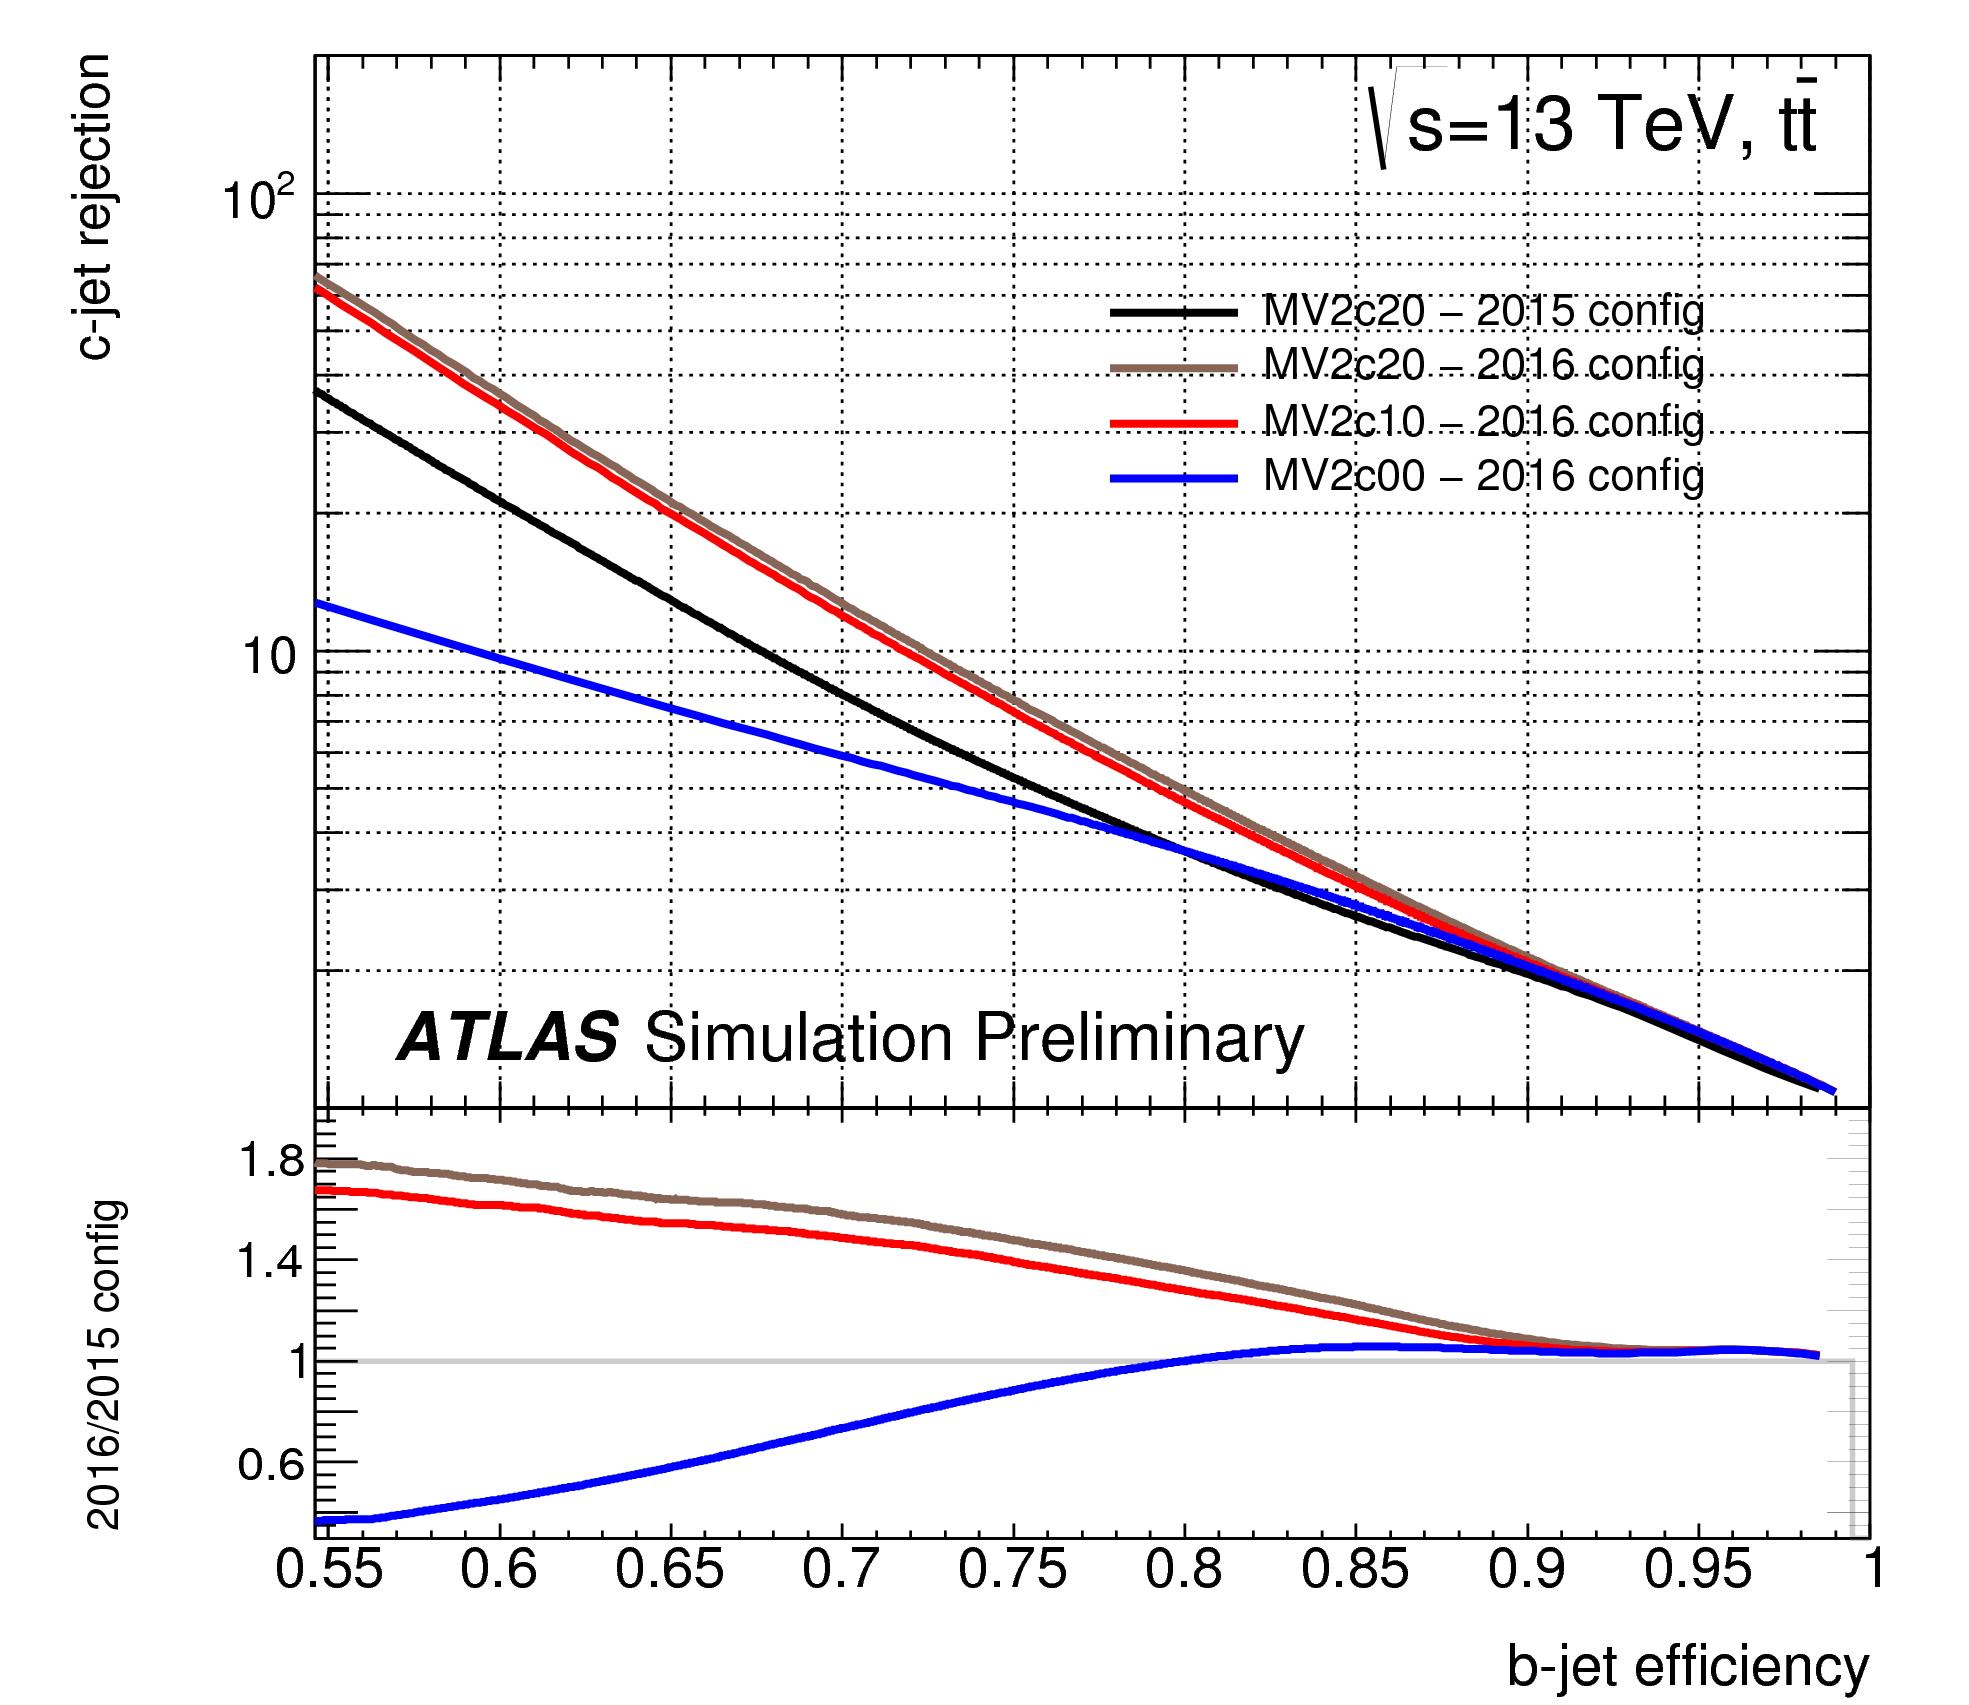
\includegraphics[width=0.48\linewidth, angle=0]{figs/Objects/bjets_perf_charm}}
  \end{center}
  \caption[The expected $b$-jet efficiency of $b$-tagging algorithm, MV2, with respect to
    (a) light-jet and (b) $c$-jet rejection in simulated $t\bar{t}$ events.
    The various lines show the performance of the algorithm for different configurations and training setups.]
    {The expected $b$-jet efficiency of $b$-tagging algorithm, MV2, with respect to
    (a) light-jet and (b) $c$-jet rejection in simulated $t\bar{t}$ events.
    The various lines show the performance of the algorithm for different configurations and training setups~\cite{obj-bjets_algo_2016}.}
  \label{fig:obj-bjets_perf}
\end{figure}

ATLAS has a set of common pre-set cuts used, known as operating points, such that work required to calibrate $b$-tagging in each analysis is shared.
Looser operating points have a relatively low cut on MV2 output, meaning that the $b$-jet efficiency is higher at the cost of worse light- and $c$-jet rejections,
and the inverse is true for tighter operating points.
Table~\ref{tab:obj-MV2_WPs} shows the list of fixed cut operating points that are used in ATLAS with a given cut on MV2c10 output;
shown with the corresponding benchmark $b$-jet efficiency, $c$-jet rejection, light-jet rejection and $\tau$ rejection.
\footnote{In this thesis only the fixed-cut operating points shown above will be used,
  however, there also exists a set of flat efficiency operating points where the MV2 cut depends on jet-\pT}
%This is in contrast to the previous multivariate tagger used in Run-1, MV1, which inputted
%the likelihood of a jet having a certain flavour from each of the three base algorithms separately.
\begin{table}[!htb]
  \begin{center}
    \begin{tabular}{|c||c|c|c|c|}
      \hline
      MV2 Cut Value  &  $b$-jet efficiency [\%]  &     $c$-jet rejection   &   Light-jet rejection  &    $\tau$ rejection  \\
      \hline
      0.9349         &           60              &           34          &      1538              &     184              \\
      0.8244         &           70              &           12          &       381              &      55              \\
      0.6459         &           77              &           6           &       134              &      22              \\
      0.1758         &           85              &           3.1         &        33              &     8.2              \\
      \hline
    \end{tabular}
    \caption[The Mv2c10 b-tagging algorithm operating points; with the corresponding $b$-jet~efficiency, $c$-jet~rejection, light-jet~rejection and $\tau$~rejection.]
            {The Mv2c10 b-tagging algorithm operating points; with the corresponding $b$-jet~efficiency, $c$-jet~rejection, light-jet~rejection and $\tau$~rejection.
              This table is taken from reference~\cite{obj-bjets_algo_2016}.}
            \label{tab:obj-MV2_WPs}
  \end{center}
  \vspace{-1cm}
\end{table}

\subsection{Calibration and Uncertainties}
\label{sec:obj-bjets_calib}

As with any part of a measurement, the process of $b$-tagging must be calibrated using data.
$b$-tagging calibration is performed using a pure sample of $b$-jets extracted from di-lepton $t\bar{t}$ events
using the probability distribution function method~\cite{obj-bjets_calib_tech,obj-bjets_calib_plots}.
With the pure $b$-jet sample one can calculate the $b$-jet efficiency, $\epsilon_{\text{bTag}}$, defined as:
\begin{equation}
 \epsilon_{\text{bTag}} = \frac{N(\text{$b$-tagged true $b$-jets)}}{N(\text{True $b$-jets)}}
\end{equation}
where $b$-tagged means above the cut on the MV2 output for a given operating point.
By measuring $\epsilon_{\text{bTag}}$ in both data and in Monte-Carlo simulation one can derive
a correction to simulation, known as a data/MC scale factor ($SF_{\text{bTag}}$), defined as:
\begin{equation}
 SF_{\text{bTag}} = \epsilon_{\text{bTag}}^{\text{Data}}/\epsilon_{\text{bTag}}^{\text{MC}}
\end{equation}
\vspace{-1em}

Uncertainties are derived for the scale factors 
to account for factors such as
uncertainties in the modelling of the backgrounds in simulation and
uncertainties in the modelling of the detector response to electrons, muons and jets.
The dominant uncertainty comes from modelling of $t\bar{t}$ in simulation.
Figure~\ref{fig:obj-bjets_calib} shows the data/MC scale factor measured in 2015 and 2016 data as a function of jet $p_T$.
The scale factor is consistent with unity within uncertainties everywhere, showing that $b$-tagging is generally well-modelled in simulation.

\begin{figure}[!ht]
  \captionsetup[subfigure]{aboveskip=-5pt,justification=centering}
  \begin{center}
    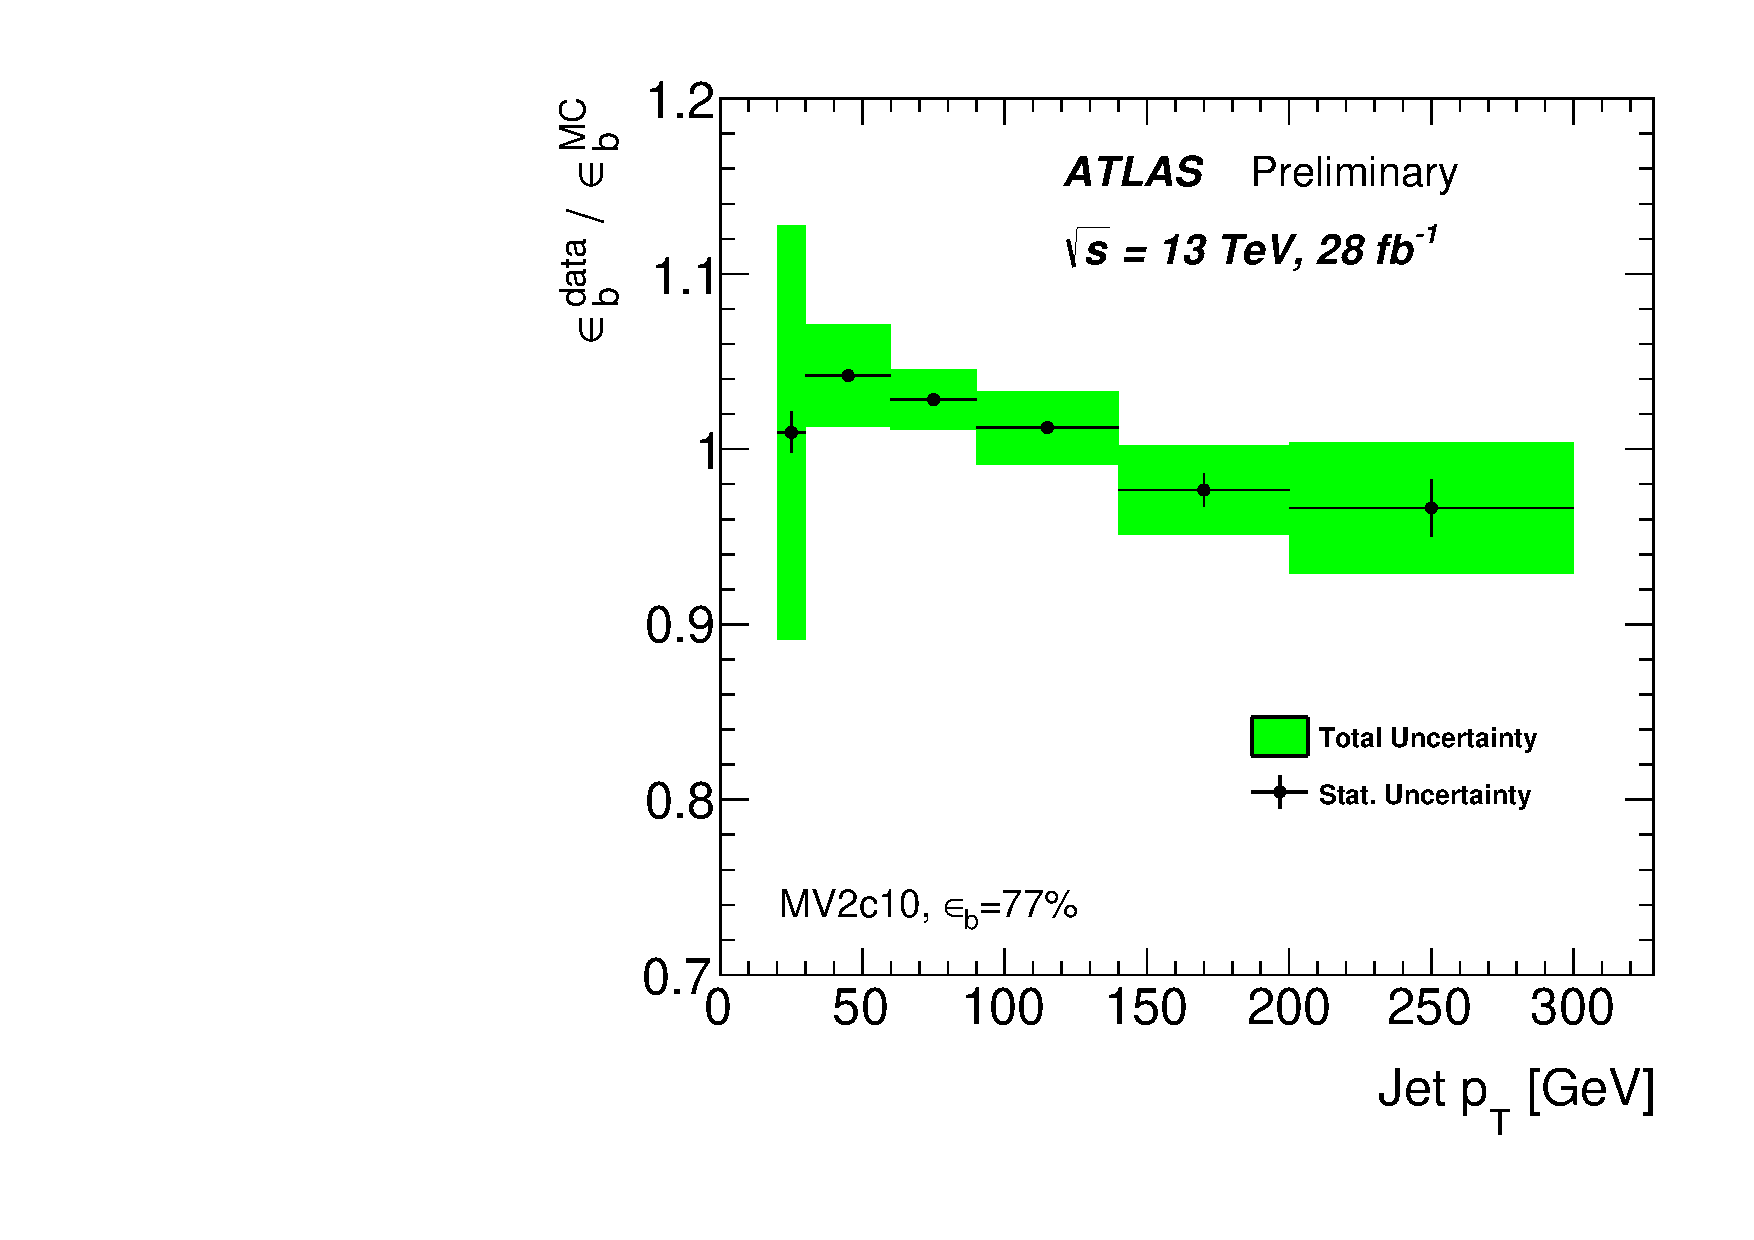
\includegraphics[width=0.7\linewidth, angle=0]{figs/Objects/bjets_calib_pt.pdf} 
  \end{center}
  \caption[Ratio of b-tagging efficiency in data and Monte Carlo for the MV2c10 b-tagging algorithm at the 77\% working point as a function of jet-$p_T$,
    extracted using di-lepton $t\bar{t}$ events. Statistical uncertainties (black lines) and total uncertainties (green shaded region) are shown.]
          {Ratio of b-tagging efficiency in data and Monte Carlo for the MV2c10 b-tagging algorithm at the 77\% working point as a function of jet-$p_T$,
    extracted using di-lepton $t\bar{t}$ events. Statistical uncertainties (black lines) and total uncertainties (green shaded region) are shown \cite{obj-bjets_calib_plots}.}
  \label{fig:obj-bjets_calib}
\end{figure}

The $b$-tagging calibration using di-lepton $t\bar{t}$ events described above
is unable to measure a data/MC scale factor for jets with $p_T$ greater than 300 GeV, due to low data statistics in the high-$p_T$ region.
Thus, the measured scale factors are extrapolated to cover the high jet-$p_T$ region, and that this extrapolation procedure introduces additional uncertainties~\cite{obj-bjets_calib_highPt}.
The extrapolation and uncertainty is calculated from simulated events by considering variations on the quantities affecting the $b$-tagging performance
such as the resolution of the impact parameter, quality of reconstructed tracks, description of the detector material, and number of tracks per jet.
The dominant effect on the uncertainty when extrapolating to the high jet-$p_T$ region is related to the different tagging efficiencies
when varying the track impact parameters. 
\textbf{Question for AK; this paragraph inspired from flag tag recommendation on a twiki; reference is internal. :/}

\clearpage
\subsection{$b$-Jet Energy Scale}
\label{sec:obj-bjets_bjes}

In Sections~\ref{sec:obj-jets_calib} and \ref{sec:obj-jets_uncert} it was described that one
must apply a correction to correct the energy of a jet from the detector-level to the true particle-level jet energy
and this correction had an associated uncertainty.
For $b$-jets this correction may be different to light jets due to differences in the parton shower and hadronisation processes for a $b$-jet;
for example during the decay of the $b$-hadron muons and neutrinos are produced which will not deposit all/any of their energy in the calorimeter
which could affect the scale of the correction. This effect is know as the $b$-jet energy scale ($b$JES) and is accounted for with an additional uncertainty.

The $b$JES uncertainty is derived and validated in data by comparing the measured jet energy with respect to a independent well calibrated object,
in this case tracks, as described in Appendix H of~\cite{dibjet-int_mori16}.
We perform this comparison for $b$-jets and inclusive jets for a dijet sample in simulation and data,
where a $b$-jet means it has been $b$-tagged at the 85\% operating point and inclusive means no requirement on $b$-tagging has been applied. 
To do the track-jet comparison tracks are associated to jets using ghost association.
Ghost association re-runs the jet clustering algorithm used to form the jets in an event,
using tracks with $p_T$ manually set to 0 as inputs in addition to the usual calorimeter topoclusters.
As the tracks have $p_T$ set to 0, the jet reconstruction algorithm will form the same jets as before,
except that tracks will now be associated to the various jets.

The measured jet-$p_T$ is compared to the sum of the tracks associated to the jet, $\Sigma p_T^{trk}$
using the observable, $r_{trk}$, defined as
\begin{equation} 
  r_{trk} = \Sigma p_{T}^{trk}/p_{T}^{jet}
\end{equation}
One can split up the expected value of the observable $r_{trk}$ into three components.
\begin{equation} 
  <r_{trk}> = <\frac{\Sigma p_{T}^{trk,truth}}{\Sigma p_{T}^{trk,reco}}> <\frac{p_{T}^{jet,truth}}{\Sigma p_{T}^{trk,truth}}> <\frac{p_{T}^{jet,reco}}{p_{T}^{jet,truth}}> 
\end{equation}
The first term describes the track energy response which, as tracks are calibrated, has been measured in data and simulation.
The second term is the mean charged fraction of the jet, $<f_{charge}>$, which will be estimated from simulation.
The third term is the jet energy response, which is the jet energy scale correction that we are interested in measuring.

The systematic uncertainties that cover the measurement of $r_{trk}$
arise from the jet and $b$-jet modelling in simulation (referred to as fragmentation),
$b$-tagging calibration, jet resolution and tracking efficiency.
In addition, an uncertainty to cover a bias observed in $<f_{charge}>$ for $b$-tagged jets relative to inclusive jets is added to the relative systematic uncertainty.
The uncertainty on the $r_{trk}$ measurement are used as the $b$JES uncertainty, which varies between 1-4\% depending on jet-$p_T$.
Figure~\ref{fig:obj-bjets_bJES_uncert} shows the derived total $b$JES uncertainty with respect to jet-$p_T$,
the components that contribute to the uncertainty are also shown.
\begin{figure}[!ht]
  \captionsetup[subfigure]{aboveskip=-5pt,justification=centering}
  \begin{center}
    \includegraphics[width=0.6\linewidth, angle=0]{figs/Objects/bjets_bJES_uncert_edit.pdf}
  \end{center}
  \caption[The total fractional $b$JES uncertainty shown with the various contributions.]
          {The total fractional $b$JES uncertainty shown with the various contributions~\cite{dibjet-int_mori16}.}
          \label{fig:obj-bjets_bJES_uncert}
\end{figure}

Then one can can test the derived $b$JES uncertainties in data using a double ratio approach.
The first ratio compares the observable in data and Monte-Carlo;
\begin{equation} 
  R_{trk} = r_{trk}^{Data}/r_{trk}^{MC}
\end{equation}
And then the double ratio, $R'_{trk}$ compares the $R_{trk}$ for $b$-jets and inclusive jets;
\begin{equation} 
  R'_{trk} = R_{trk}^{b-\text{jet}}/R_{trk}^{\text{incl.}}
\end{equation}
The double-ratio approach means that many of the uncertainties unrelated to $b$JES are cancelled in the ratios.

Figure~\ref{fig:obj-bjets_bJES_Rprime} shows the double ratio $R'_{trk}$ with the $b$JES uncertainty applied.
The ratio is almost consistent with unity within uncertainties validating our $b$JES uncertainty in data.

  \begin{figure}[!ht]
  \begin{center}
      \includegraphics[width=0.6\linewidth, angle=0]{figs/Objects/bjets_bJES_Rprime_edit.pdf}
  \end{center}
  \caption[The validation of the $b$JES uncertainty in data using the double-ratio $R'_{trk}$.]
          {The validation of the $b$JES uncertainty in data using the double-ratio $R'_{trk}$~\cite{dibjet-int_mori16}.}
  \label{fig:obj-bjets_bJES_Rprime}
\end{figure}






%\section{bTagging: Validation in Dijet Events}

\newpage
\section{Electrons and Muons}
\label{sec:obj-leptons}

Reconstruction of electrons and muons
is important for a number of analyses at ATLAS;
including the selection of di-lepton $t\bar{t}$ events
which are used in the calibration of $b$-tagging and the $b$-jet trigger,
described in Sections~\ref{sec:obj-bjets_calib} and~\ref{sec:trig-bjet_eff} respectively.
As these objects are not used in the final analysis presented in this thesis,
they are described below in less detail than has been given to jets and $b$-jets.

Electron\footnote{For the purposes of reconstruction positrons are included as a subset of electrons}
reconstruction at ATLAS ~\cite{obj-electrons} uses
the matching of narrow clusters of energy deposits in the calorimeter
to a track from the inner detector,
from which the four-momentum of the electron can be determined.
Information such as the calorimeter shower shape,
properties of the matched track
and TRT transition radiation (described in Section~\ref{sec:det-ID})
allows for identification of electrons with respect to other physics objects described in this section.
Three different operating points are provided for electron identification:
which are, in order of increasing background rejection
\textit{Loose}, \textit{Medium}, and \textit{Tight}. 

Muon\footnote{Similar to positrons, in reconstruction anti-muons are included as a subset of muons}
reconstruction at ATLAS  uses muon tracks reconstructed using the Muon Spectrometer (MS) and tracks constructed by the Inner Detector (ID).
There are several types of muon reconstruction techniques
and different muon identification working points available~\cite{obj-muons}.

Two of the techniques for reconstruction are combined muons and extrapolated muons.
Combined muons are reconstructed by extrapolating muon tracks inwards to match tracks formed by the ID.
Extrapolated muons are formed from muon tracks alone,
with a loose requirement on the track pointing to the primary vertex;
extrapolated muons are important in the range $2.5 < \eta < 2.7$ for which there is no ID coverage.
Again for reconstructed muons the four-momentum can be determined.

Four muon identification working points have been defined \textit{Loose}, \textit{Medium}, \textit{Tight}, and \textit{High-$p_T$}.
Medium muons, as used in Section~\ref{sec:trig-bjet_eff}, are made up of combined and extrapolated muons that pass a quality criteria based on
number of MS hits, track fit quality and, where relevant, compatibility between the ID and MS tracks.

\section{Further objects}
\label{sec:obj-further}

In the previous sections of this chapter all objects used in the analyses presented in this analysis have been described.
However this is not an exhaustive list of the range of objects that ATLAS can reconstruct.
In this section I will briefly outline some of the many other objects of interest that are used elsewhere in ATLAS analyses.

\begin{itemize}[leftmargin=*]
\item\textbf{Photons:}
  Photons can be identified from using narrow clusters of energy deposits in the calorimeter similar to that of electrons,
  except with no track associated~\cite{obj-photons}.
  Information such as the calorimeter shower shape and TRT transition radiation
 allows for identification of electrons with respect to other physics objects, notably electrons.\vspace{0.5em}
\item\textbf{Taus:}
  Taus, in their most common decay mode, can be identified and reconstructed using narrow calorimeter jets
  associated to a topologies of tracks that match their known decay chain~\cite{obj-taus}.\vspace{0.5em}
\item\textbf{Missing Transverse Momentum:}
  It is known that the momentum in the transverse plane is conserved,
  hence from the negative sum of the momentums of all reconstructed physics objects in an event
  one can determine the presence of missing transverse momentum (MET)~\cite{obj-met}.
  MET can be used to identify the presence of particles that interact weakly with the ATLAS detector,
  such as neutrinos~\cite{obj-Hbb} or even dark matter~\cite{obj-met_monoJet}.
\end{itemize}
